\documentclass[xcolor=dvipsnames]{beamer}
\usepackage{lmodern}
\usepackage[T1]{fontenc}
\usepackage[english]{babel}
\usepackage[utf8]{inputenc}

\usepackage{manfnt}
\usepackage{wasysym}
\usepackage{listings}
\usepackage{graphicx}
\usepackage{url}
\usepackage{ulem}
\usepackage{marvosym}
\usepackage{skull}
\usepackage{proof}
\usepackage{array}
\setbeamertemplate{navigation symbols}{}

\title[Landslide]{{\bf Landslide: Systematic Dynamic Race Detection in Kernel-space}}
\subtitle[]{ {\em showing that Pebbles are less stable than you thought since 2011.}}
\author[Ben Blum]{Ben Blum \texttt{(bblum@andrew.cmu.edu)}}

\institute[CMU]{Carnegie Mellon University}
\date[]{2012, May 10}

\setbeamertemplate{footline}{\hspace*{.5cm}\scriptsize{\insertauthor\hspace*{50pt} \hfill\insertframenumber\hspace*{.5cm}}} 

\usecolortheme{seahorse}
\usecolortheme{rose}
\useoutertheme{infolines}

\usecolortheme[named=RoyalBlue]{structure}

\newcommand\noob{\mathsf{noob}}
\newcommand\gibs{\mathsf{gibs}}
\newcommand\dps{\mathsf{dps}}
\newcommand\squig\rightsquigarrow
\newcommand\Coloneqq{\mathrel{\mathop{::}}=}
\newcommand\dmg{\text{\Laserbeam}}
\newcommand\delter\delta
\newcommand\alpher\alpha
\newcommand\defnor{\text{ }|\text{ }}

\newcommand\pimp{\mathop{\supset}}
\newcommand\pand{\mathop{\wedge}}
\newcommand\por{\mathop{\vee}}
\newcommand\ptrue{\top}
\newcommand\pfalse{\bot}


\begin{document}
\normalem
\begin{frame}
	\titlepage
\end{frame}

%%%%%%%%%%%%%%%%%%%%%%%%%%%%%%%%%%%%%%%%%%%%%%%%%%%%%%%%%%%%%%%%%%%%%%%%%%%%%%%%
%%%%%%%%%%%%%%%%%%%%%%%%%%%%%%%%%%%%%%%%%%%%%%%%%%%%%%%%%%%%%%%%%%%%%%%%%%%%%%%%
%%%%%%%%%%%%%%%%%%%%%%%%%%%%%%%%%%%%%%%%%%%%%%%%%%%%%%%%%%%%%%%%%%%%%%%%%%%%%%%%

\newcommand\linegap{\vspace{0.2in}}
\newcommand\breakslide[1]{\begin{frame}{} \begin{center} #1 \end{center} \end{frame}}
\newcommand\related[1]{\textsuperscript{\em [#1]}}

\begin{frame}{Outline}
	\textbf{Motivation: Concurrency debugging}
	\begin{itemize}
		\item Systematic exploration versus stress testing
		\item Challenges of kernel-space
	\end{itemize}
	\linegap

	{\bf Tool: Landslide}
	\begin{itemize}
		\item Design and interface
		\item Addressing challenges
	\end{itemize}
	\linegap

	{\bf Evaluation: Finding Races}
	\begin{itemize}
		\item Student user study
		\item Case study
	\end{itemize}
	\linegap

	{\bf Future Work and Conclusion}
\end{frame}

%%%%%%%%%%%%%%%%%%%%%%%%%%%%%%%%%%%%%%%%%%%%%%%%%%%%%%%%%%%%%%%%%%%%%%%%%%%%%%%%
\section{Motivation}
%%%%%%%%%%%%%%%%%%%%%%%%%%%%%%%%%%%%%%%%%%%%%%%%%%%%%%%%%%%%%%%%%%%%%%%%%%%%%%%%

%%%%%%%%%%%%%%%%%%%%%%%%%%%%%%%%%%%%%%%%%%%%%%%%%%%%%%%%%%%%%%%%%%%%%%%%%%%%%%%%
\subsection{Race Conditions and the Finding Thereof}

\begin{frame}[fragile]{Case Study}
	\begin{center}
	\begin{verbatim}
	        int thread_fork()
	        {
	            thread_t *child = spawn_new_thread();
	            add_to_runqueue(child);
	            return child->tid;
	        }
	\end{verbatim}
	\end{center}

	\begin{itemize}
		\item On exit, child's TCB is freed
		\item Forking thread does use-after-free
		\item Might return garbage instead of TID
	\end{itemize}
\end{frame}

\begin{frame}{Testing Techniques} % slide: sys ex vs stress testing
	\textbf{Stress Testing:} Common testing approach
	\begin{itemize}
		\item Attempting to exercise as many interleavings as possible
		\item Exposes race conditions at random
		\begin{itemize}
			\item ``If a preemption occurs at {\em just the right time}\dots''
		\end{itemize}
		\item Cryptic panic messages or machine reboots
	\end{itemize}
	\linegap

	{\bf Systematic Exploration} \related{Simsa '10}
	\begin{itemize}
		\item Make educated guesses about when to preempt
		\item Run {\em every single} interleaving
		\item Provide better debugging information
	\end{itemize}
\end{frame}

\begin{frame}{Execution Tree} % slide: decision tree
	\begin{center}
		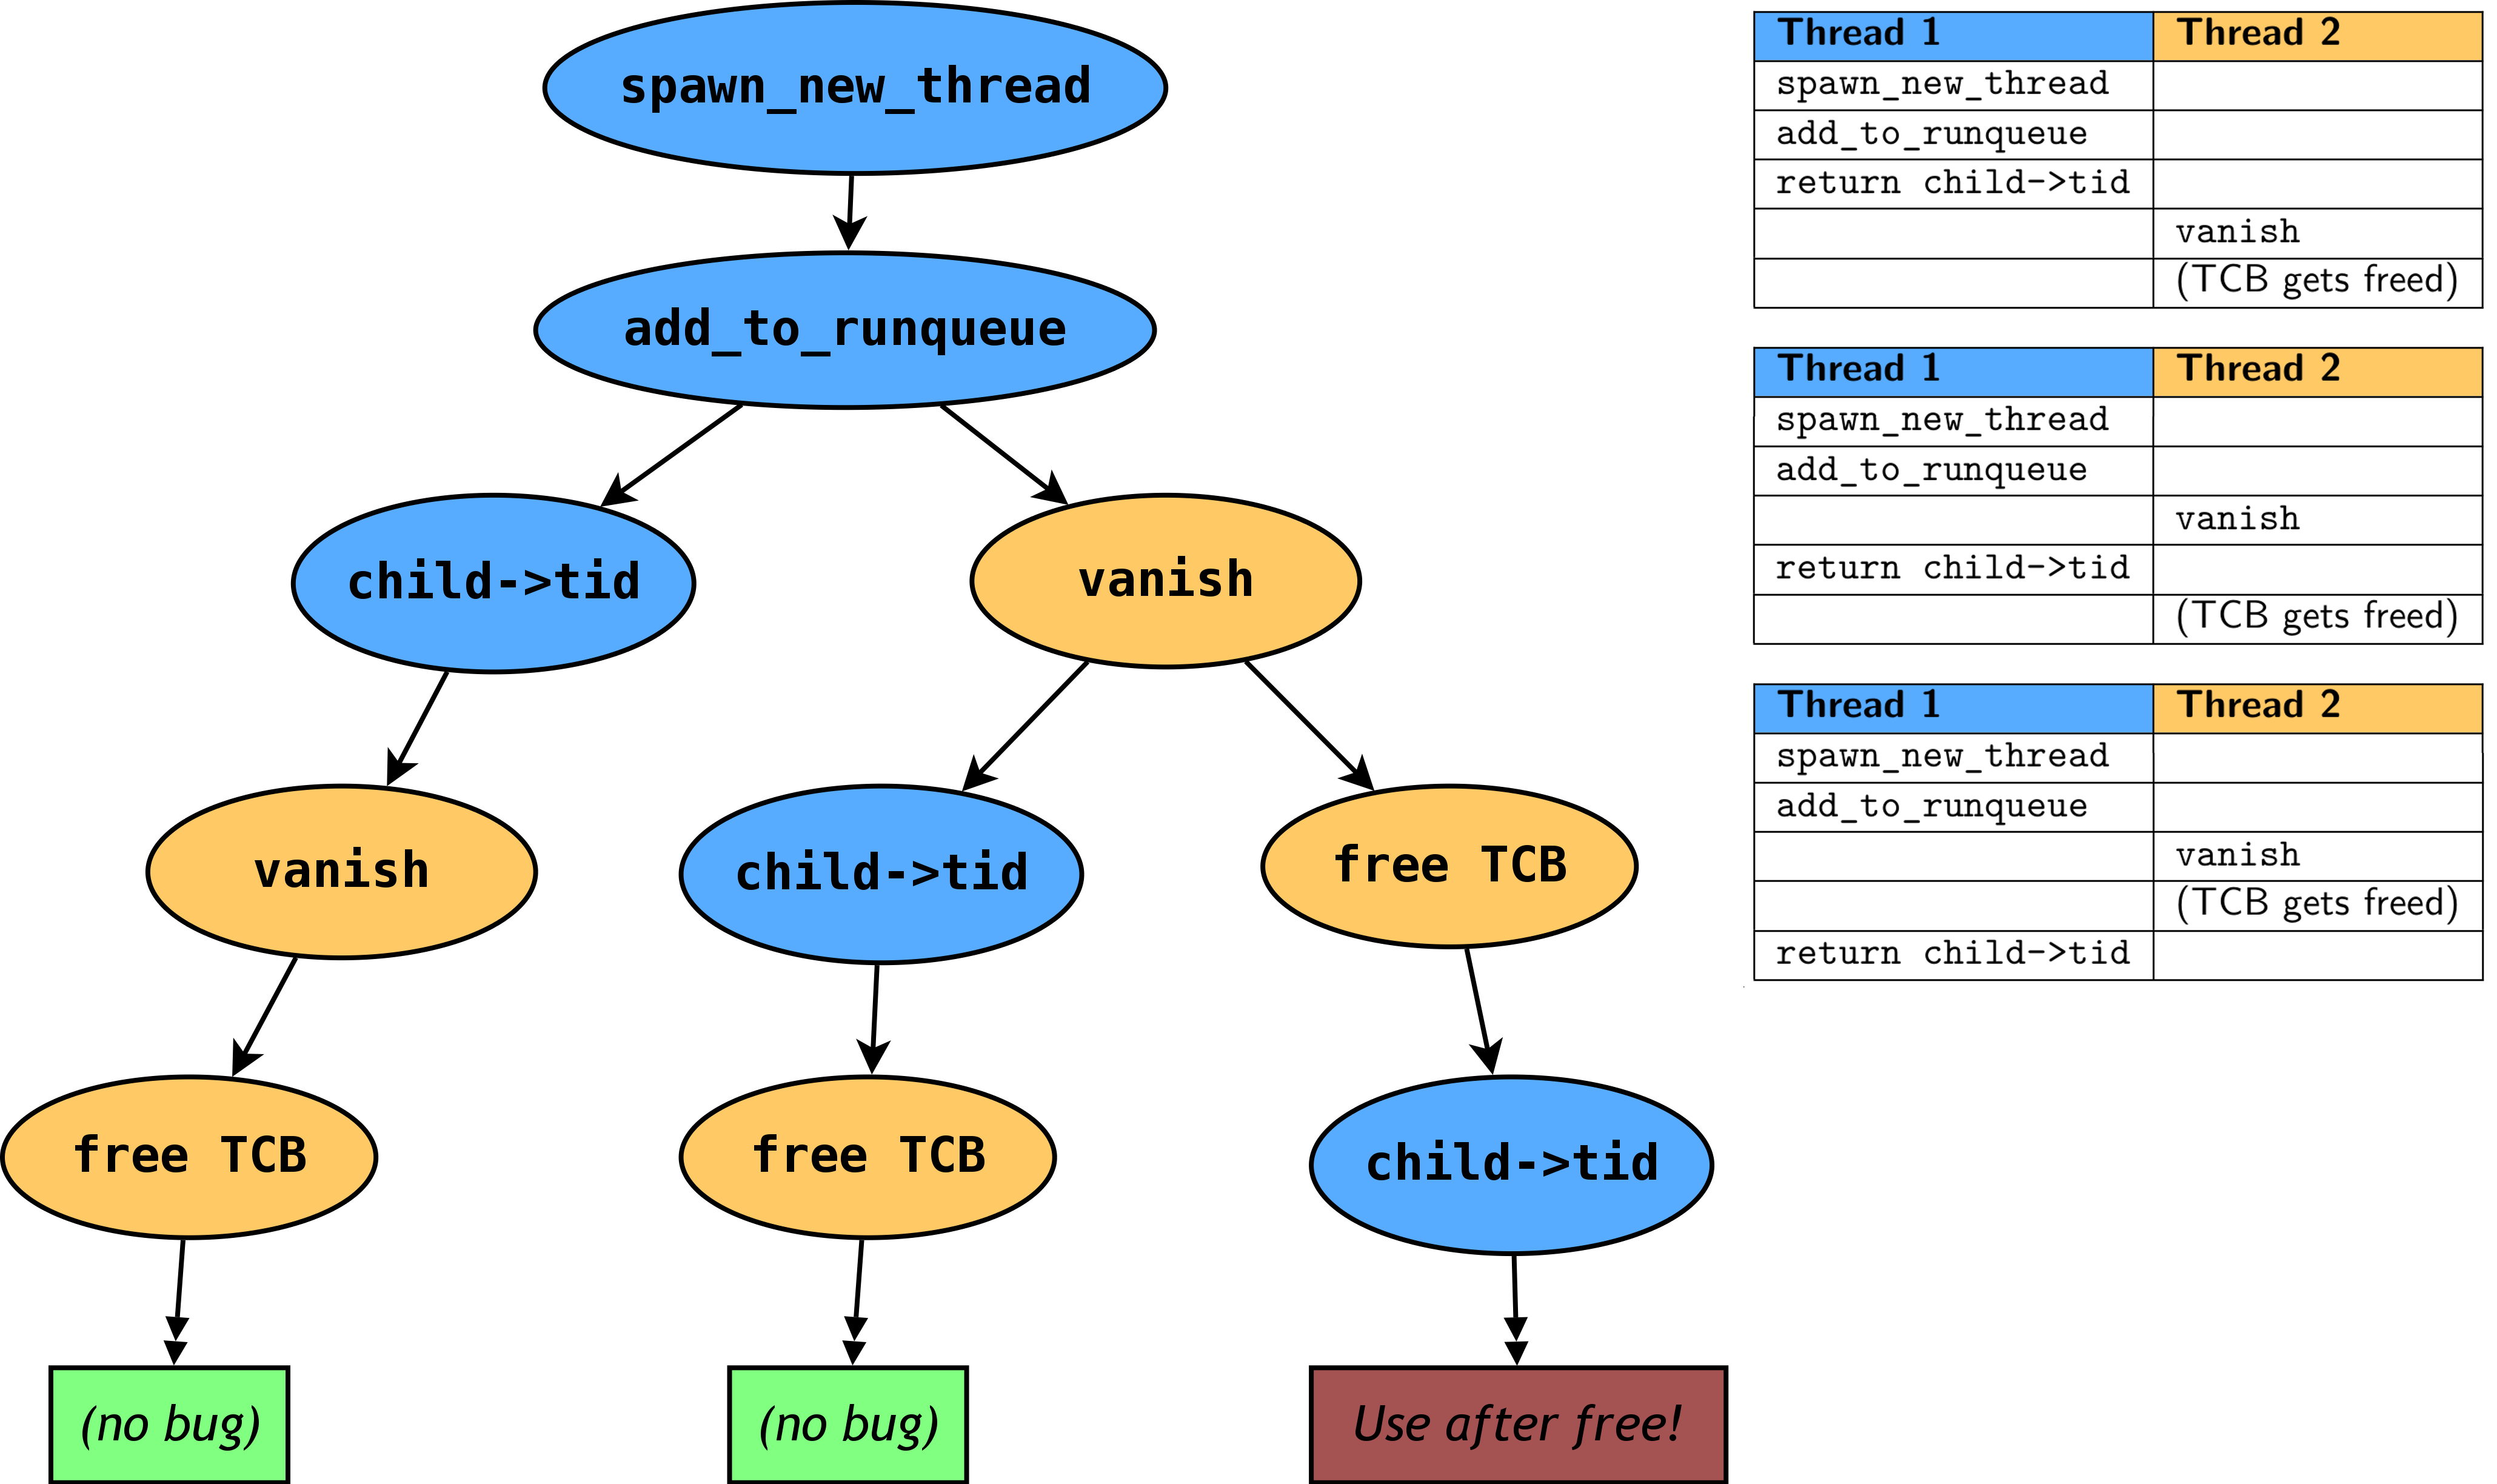
\includegraphics[width=\textwidth]{tree.png}
	\end{center}
\end{frame}

\begin{frame}{Finding Races in Kernel-Space} % slide: 15-410 6-week project why we need it in kernels
	Previous work in kernel-space has not used systematic exploration.
	\linegap

	\textbf{15-410:} Operating System Design and Implementation
	\begin{itemize}
		\item Project 3: students write a kernel in 6 weeks.
		\item ``Pebbles'' is a UNIX-like, preemptible kernel specification.
	\end{itemize}
	%\begin{itemize}
	%	\item Data race detection\related{Erickson '10}
	%	\item Failure resiliency\related{Kadav '09}
	%\end{itemize}
\end{frame}

%%%%%%%%%%%%%%%%%%%%%%%%%%%%%%%%%%%%%%%%%%%%%%%%%%%%%%%%%%%%%%%%%%%%%%%%%%%%%%%%
\subsection{Challenges of Kernel-space}

\breakslide{Why is this environment different from all other environments?}

\begin{frame}{Causes of Concurrency} % slide: causes of concurrency, thread scheduling
	\textbf{Kernels contain their own concurrency implementation.}

	\linegap
	Context switching
	\begin{itemize}
		\item Non-deterministic timer-driven thread scheduling
	\end{itemize}
	Runqueue tracking
	\begin{itemize}
		\item Which threads are runnable?
	\end{itemize}
	Thread lifecycle tracking
	\begin{itemize}
		\item When are threads created/destroyed?
	\end{itemize}
\end{frame}

% slide: ad-hoc communication, memory conflicts (freeing, runqueue)
%\begin{frame}{Ad-Hoc Thread Communication}
%	No message-passing % TODO this slide sucks
%	
%	User-space systematic exploration relies on it\related{Simsa '10}; we cannot.
%	
%	Kernel threads share state via globals, heap.
%\end{frame}

\begin{frame}{The Kernel as One Program} % slide: the kernel is too big to test all at once
	\begin{center}
	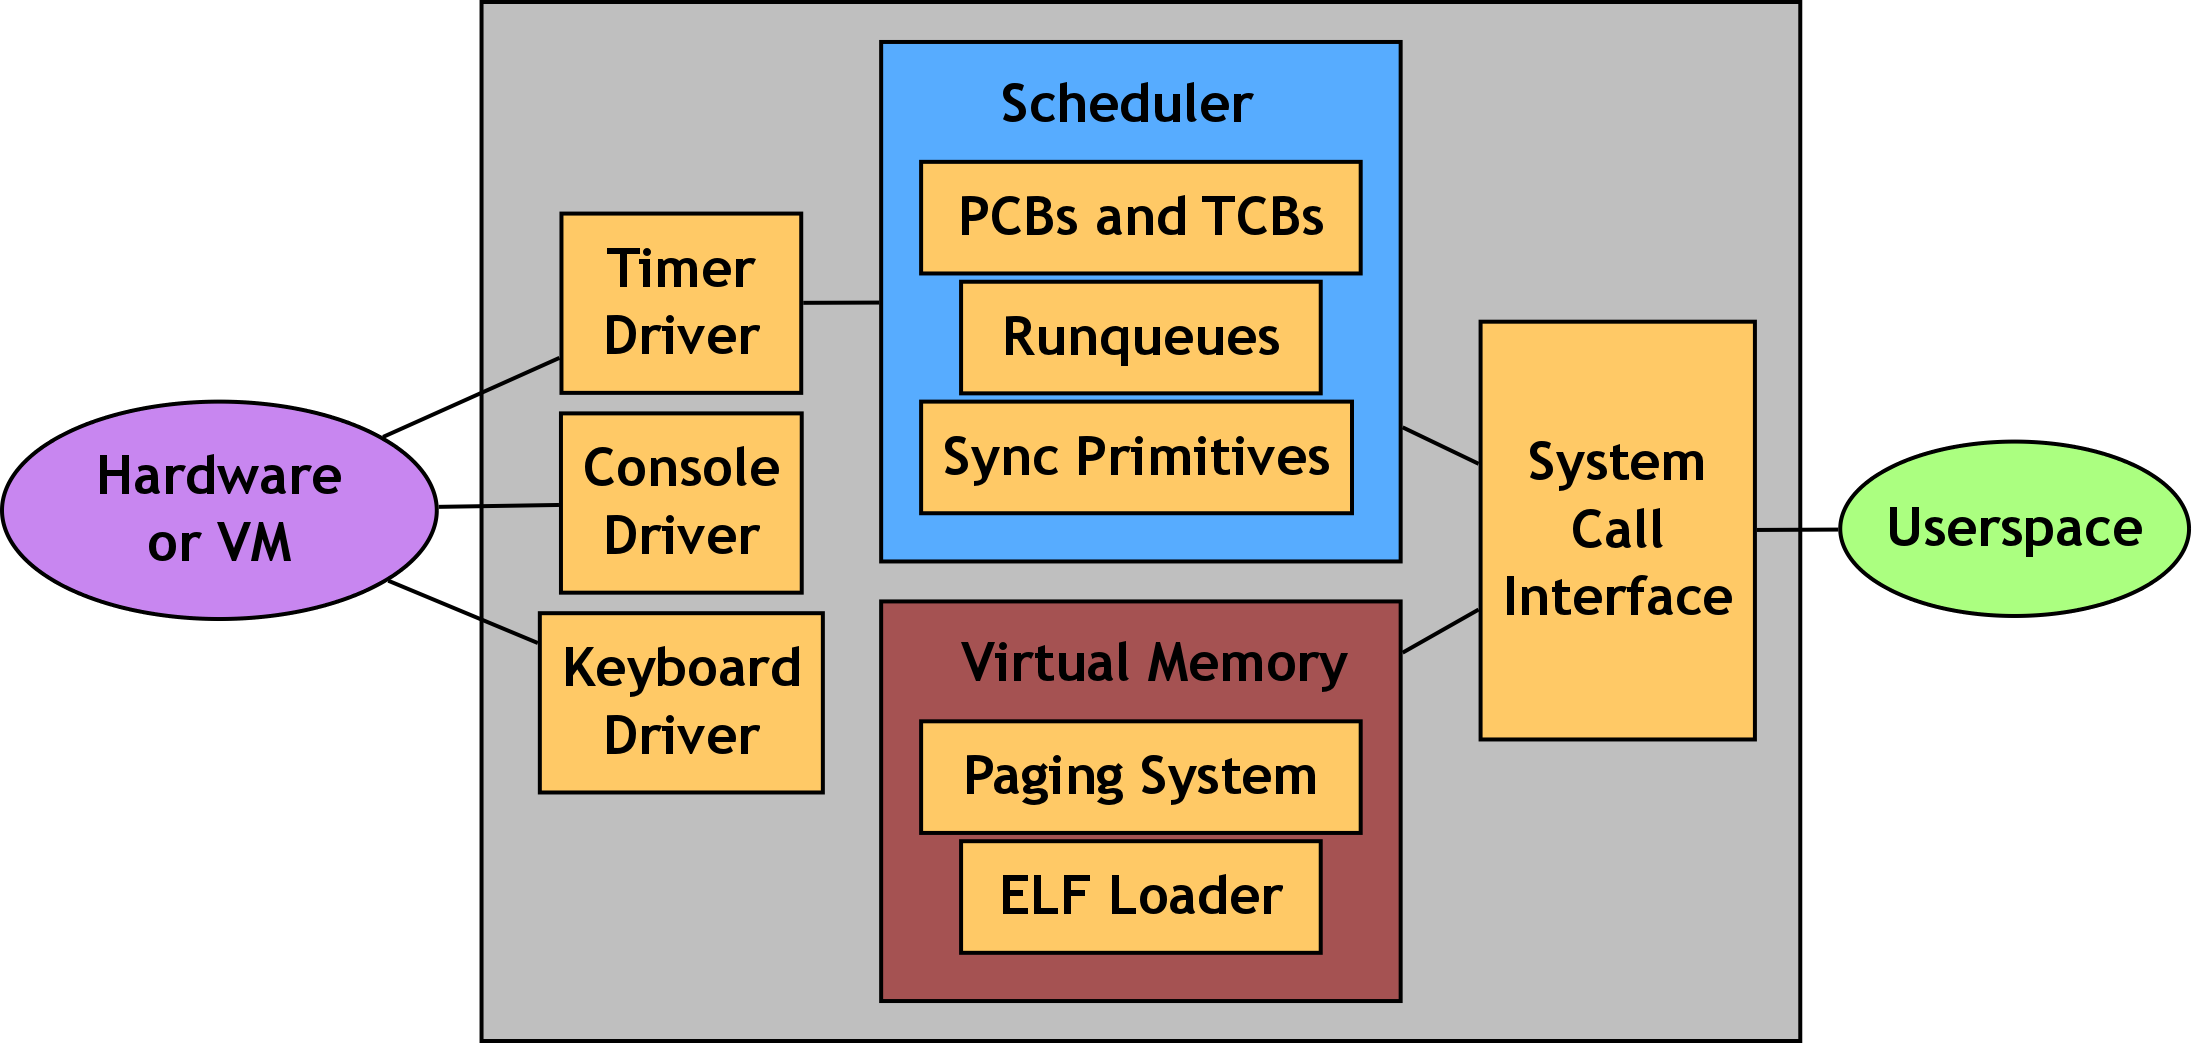
\includegraphics[width=\textwidth]{pebbles.png}
	\end{center}
\end{frame}
\begin{frame}{The Kernel as One Program} % slide: the kernel is too big to test all at once
	\begin{itemize}
		\item ``Everything interleaves with everything else''?
		\item What is a ``bug'', anyway?\related{Baumann '09}
	\end{itemize}
	% Say: "we don't want to have to explore every possible interaction between each of these components"
\end{frame}

\begin{frame}{Contribution} % slide: summary: "sys ex is a tool \ldots``
	Systematic exploration is a {\em tool} for testing concurrent systems.
	\begin{itemize}
		\item How can it be applied in kernel-space?
		\item What can we ask of the user to make it possible?
	\end{itemize}
	\linegap

	{\bf Landslide} is an effort to answer these questions.
	% say: landslide is an exploratory work into finding out what lies behind these questions.
\end{frame}

%%%%%%%%%%%%%%%%%%%%%%%%%%%%%%%%%%%%%%%%%%%%%%%%%%%%%%%%%%%%%%%%%%%%%%%%%%%%%%%%
\section{Landslide}
%%%%%%%%%%%%%%%%%%%%%%%%%%%%%%%%%%%%%%%%%%%%%%%%%%%%%%%%%%%%%%%%%%%%%%%%%%%%%%%%

\newcommand\done[1]{\textcolor{gray}{\em \small #1}}

%\begin{frame}{Outline}
%	\done{Motivation: Concurrency debugging}
%	\begin{itemize}
%		\item \done{Systematic exploration versus stress testing}
%		\item \done{Challenges of kernel-space}
%	\end{itemize}
%	\linegap
%
%	{\bf Tool: Landslide}
%	\begin{itemize}
%		\item {\bf Design and interface}
%		\item {\bf Addressing challenges}
%	\end{itemize}
%	\linegap
%
%	Evaluation: Finding Races
%	\begin{itemize}
%		\item Student user study
%		\item Case study
%	\end{itemize}
%	\linegap
%
%	Future Work and Conclusion
%\end{frame}

%%%%%%%%%%%%%%%%%%%%%%%%%%%%%%%%%%%%%%%%%%%%%%%%%%%%%%%%%%%%%%%%%%%%%%%%%%%%%%%%
\subsection{Design}

\begin{frame}{Environment}
	\textbf{Simics:} a full-system x86 simulator
	\begin{itemize}
		\item Students in 15-410 use Simics to test their kernels.
		\item Landslide is a transparently-embedded Simics module.
	\end{itemize}
\end{frame}

\begin{frame}{Anatomy of Landslide}
	\begin{center}
	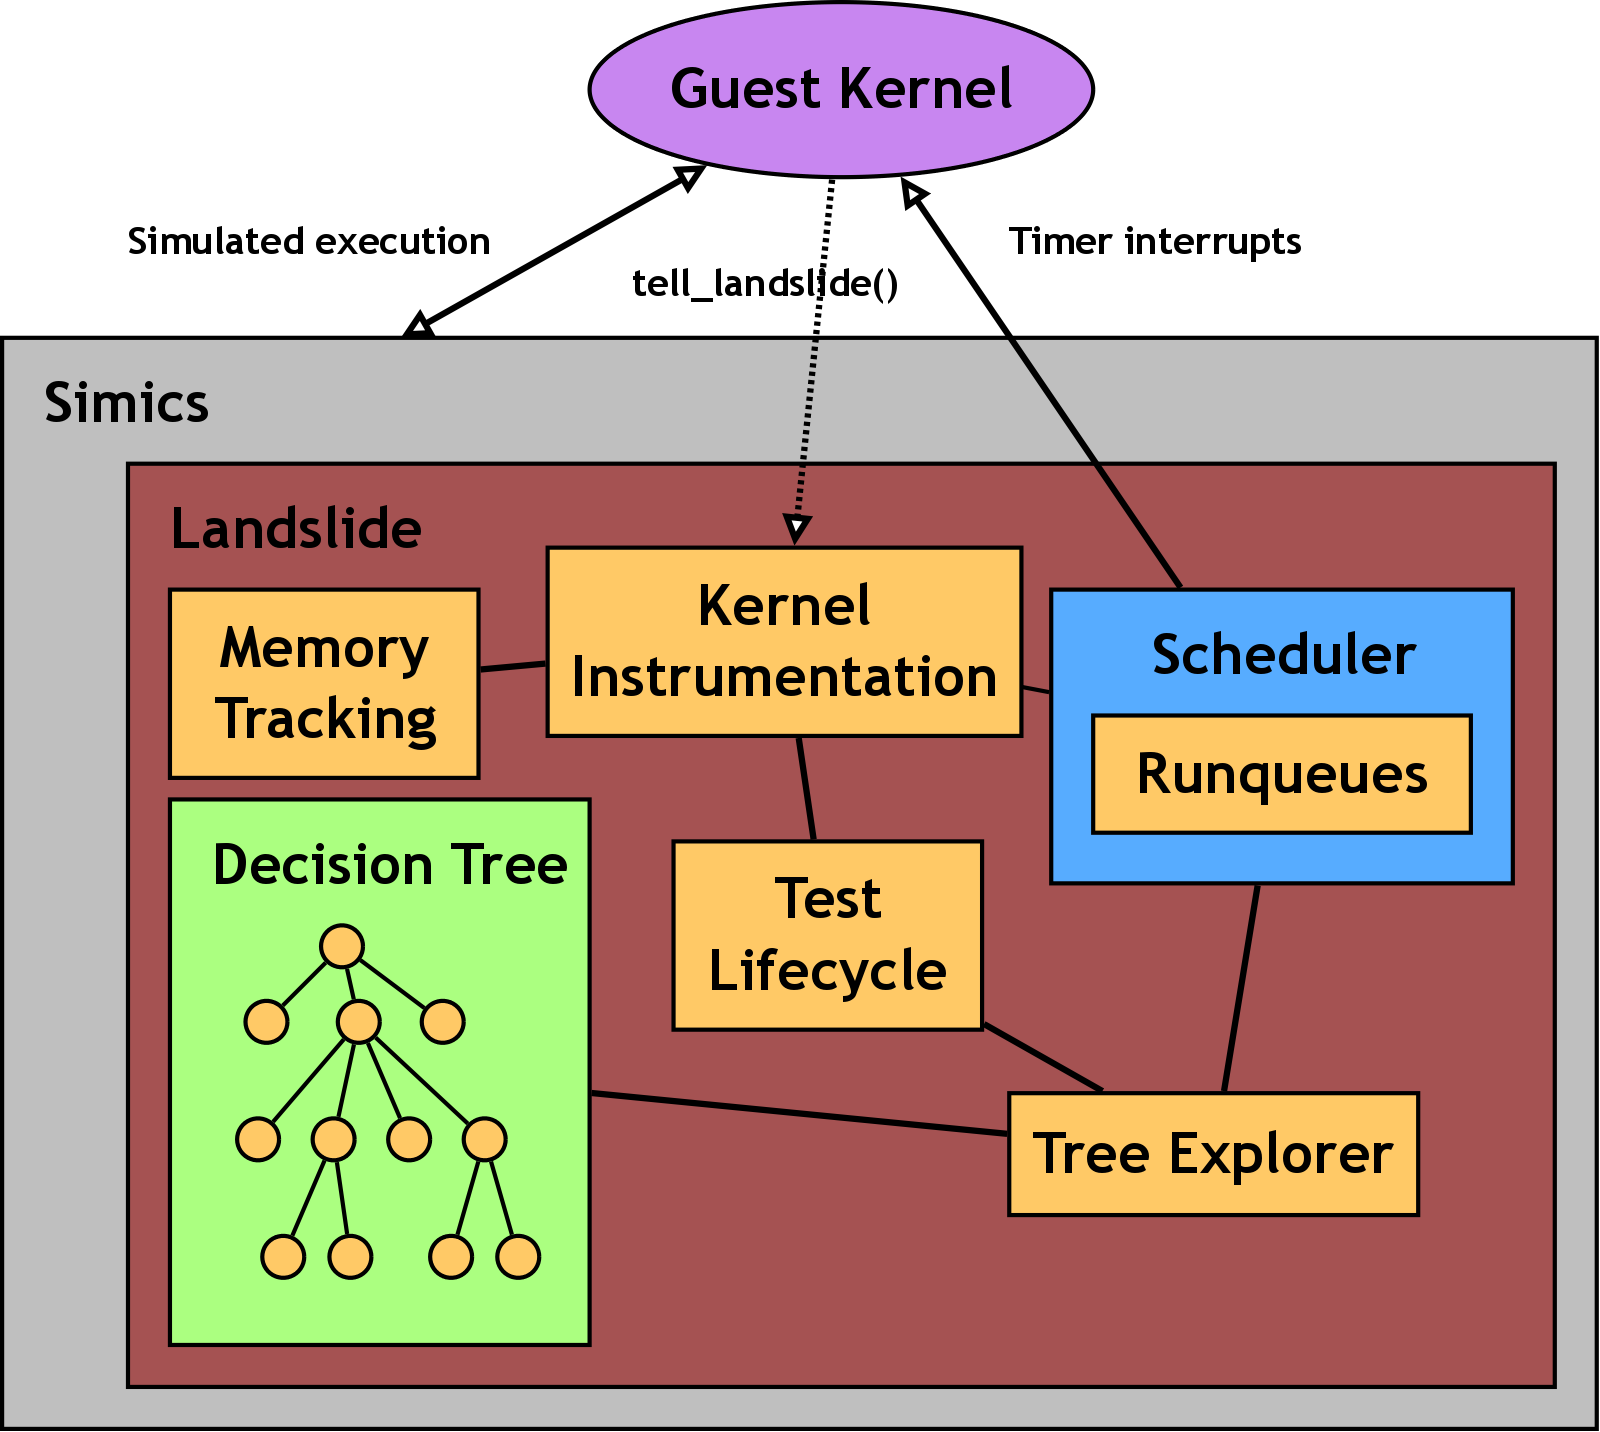
\includegraphics[width=0.7\textwidth]{landslide.png}
	\end{center}
	% Remember to talk about solving the thread scheduling challenge
\end{frame}

\subsection{Interface}

\begin{frame}{Using Landslide}
	\begin{center}
	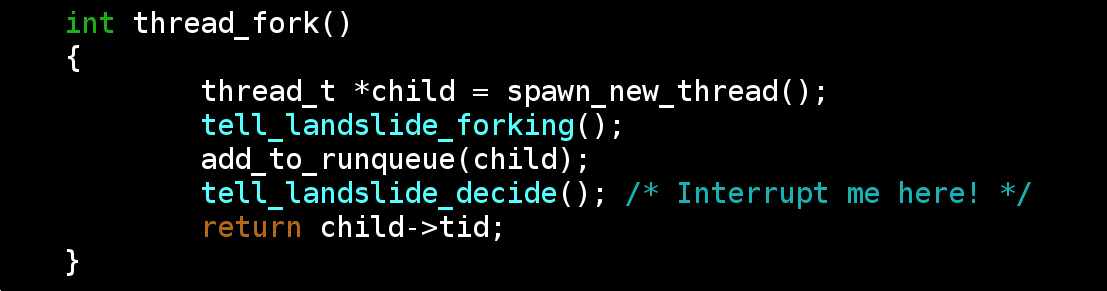
\includegraphics[width=0.9\textwidth]{tell_landslide.png}
	\end{center}
	User must tell Landslide when certain kernel events happen:
	\begin{itemize}
		\item When do threads become runnable / descheduled?
		\item When does the scheduler switch threads?
	\end{itemize}
	\linegap
	% TODO
	Some complicated conditions require in-Landslide instrumentation.
	\begin{itemize}
		\item Scheduler design details
	\end{itemize}
\end{frame}

\begin{frame}{Decision Trace}
	% FIXME make the stack trace coloured
	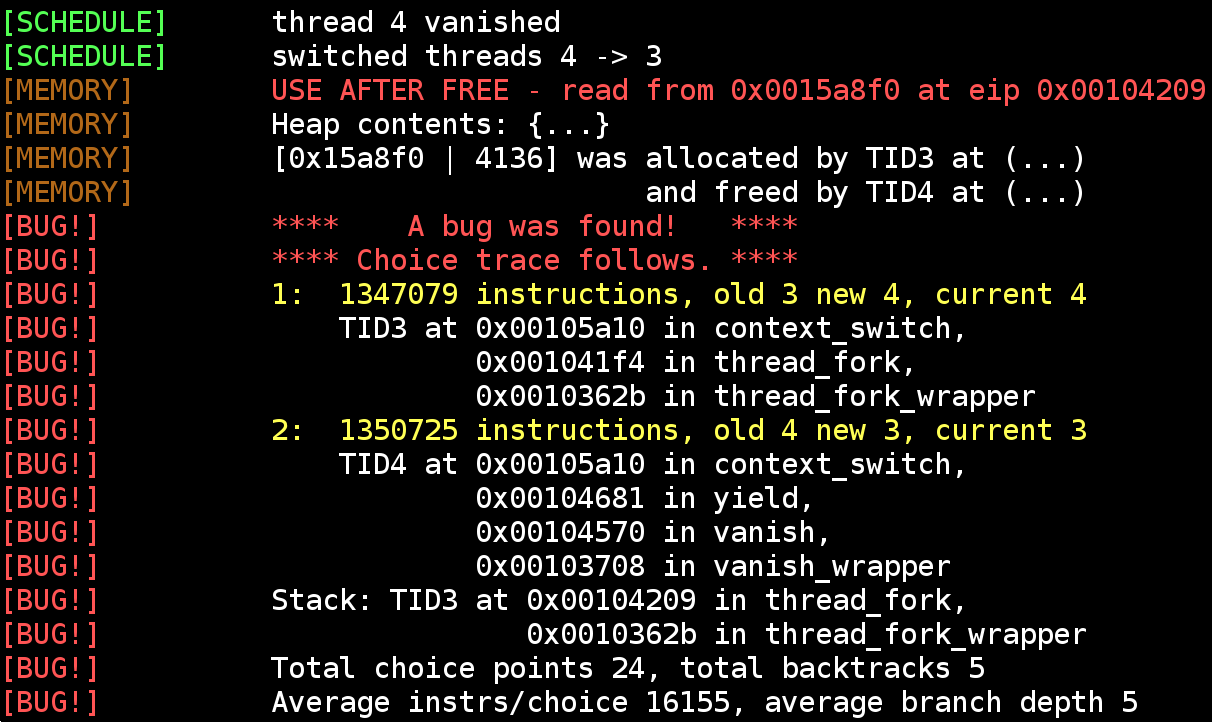
\includegraphics[width=\textwidth]{found_a_bug.png}
\end{frame}

%%%%%%%%%%%%%%%%%%%%%%%%%%%%%%%%%%%%%%%%%%%%%%%%%%%%%%%%%%%%%%%%%%%%%%%%%%%%%%%%
\subsection{Addressing Challenges} % rename

\begin{frame}{State Space Reduction}
	\begin{center}
	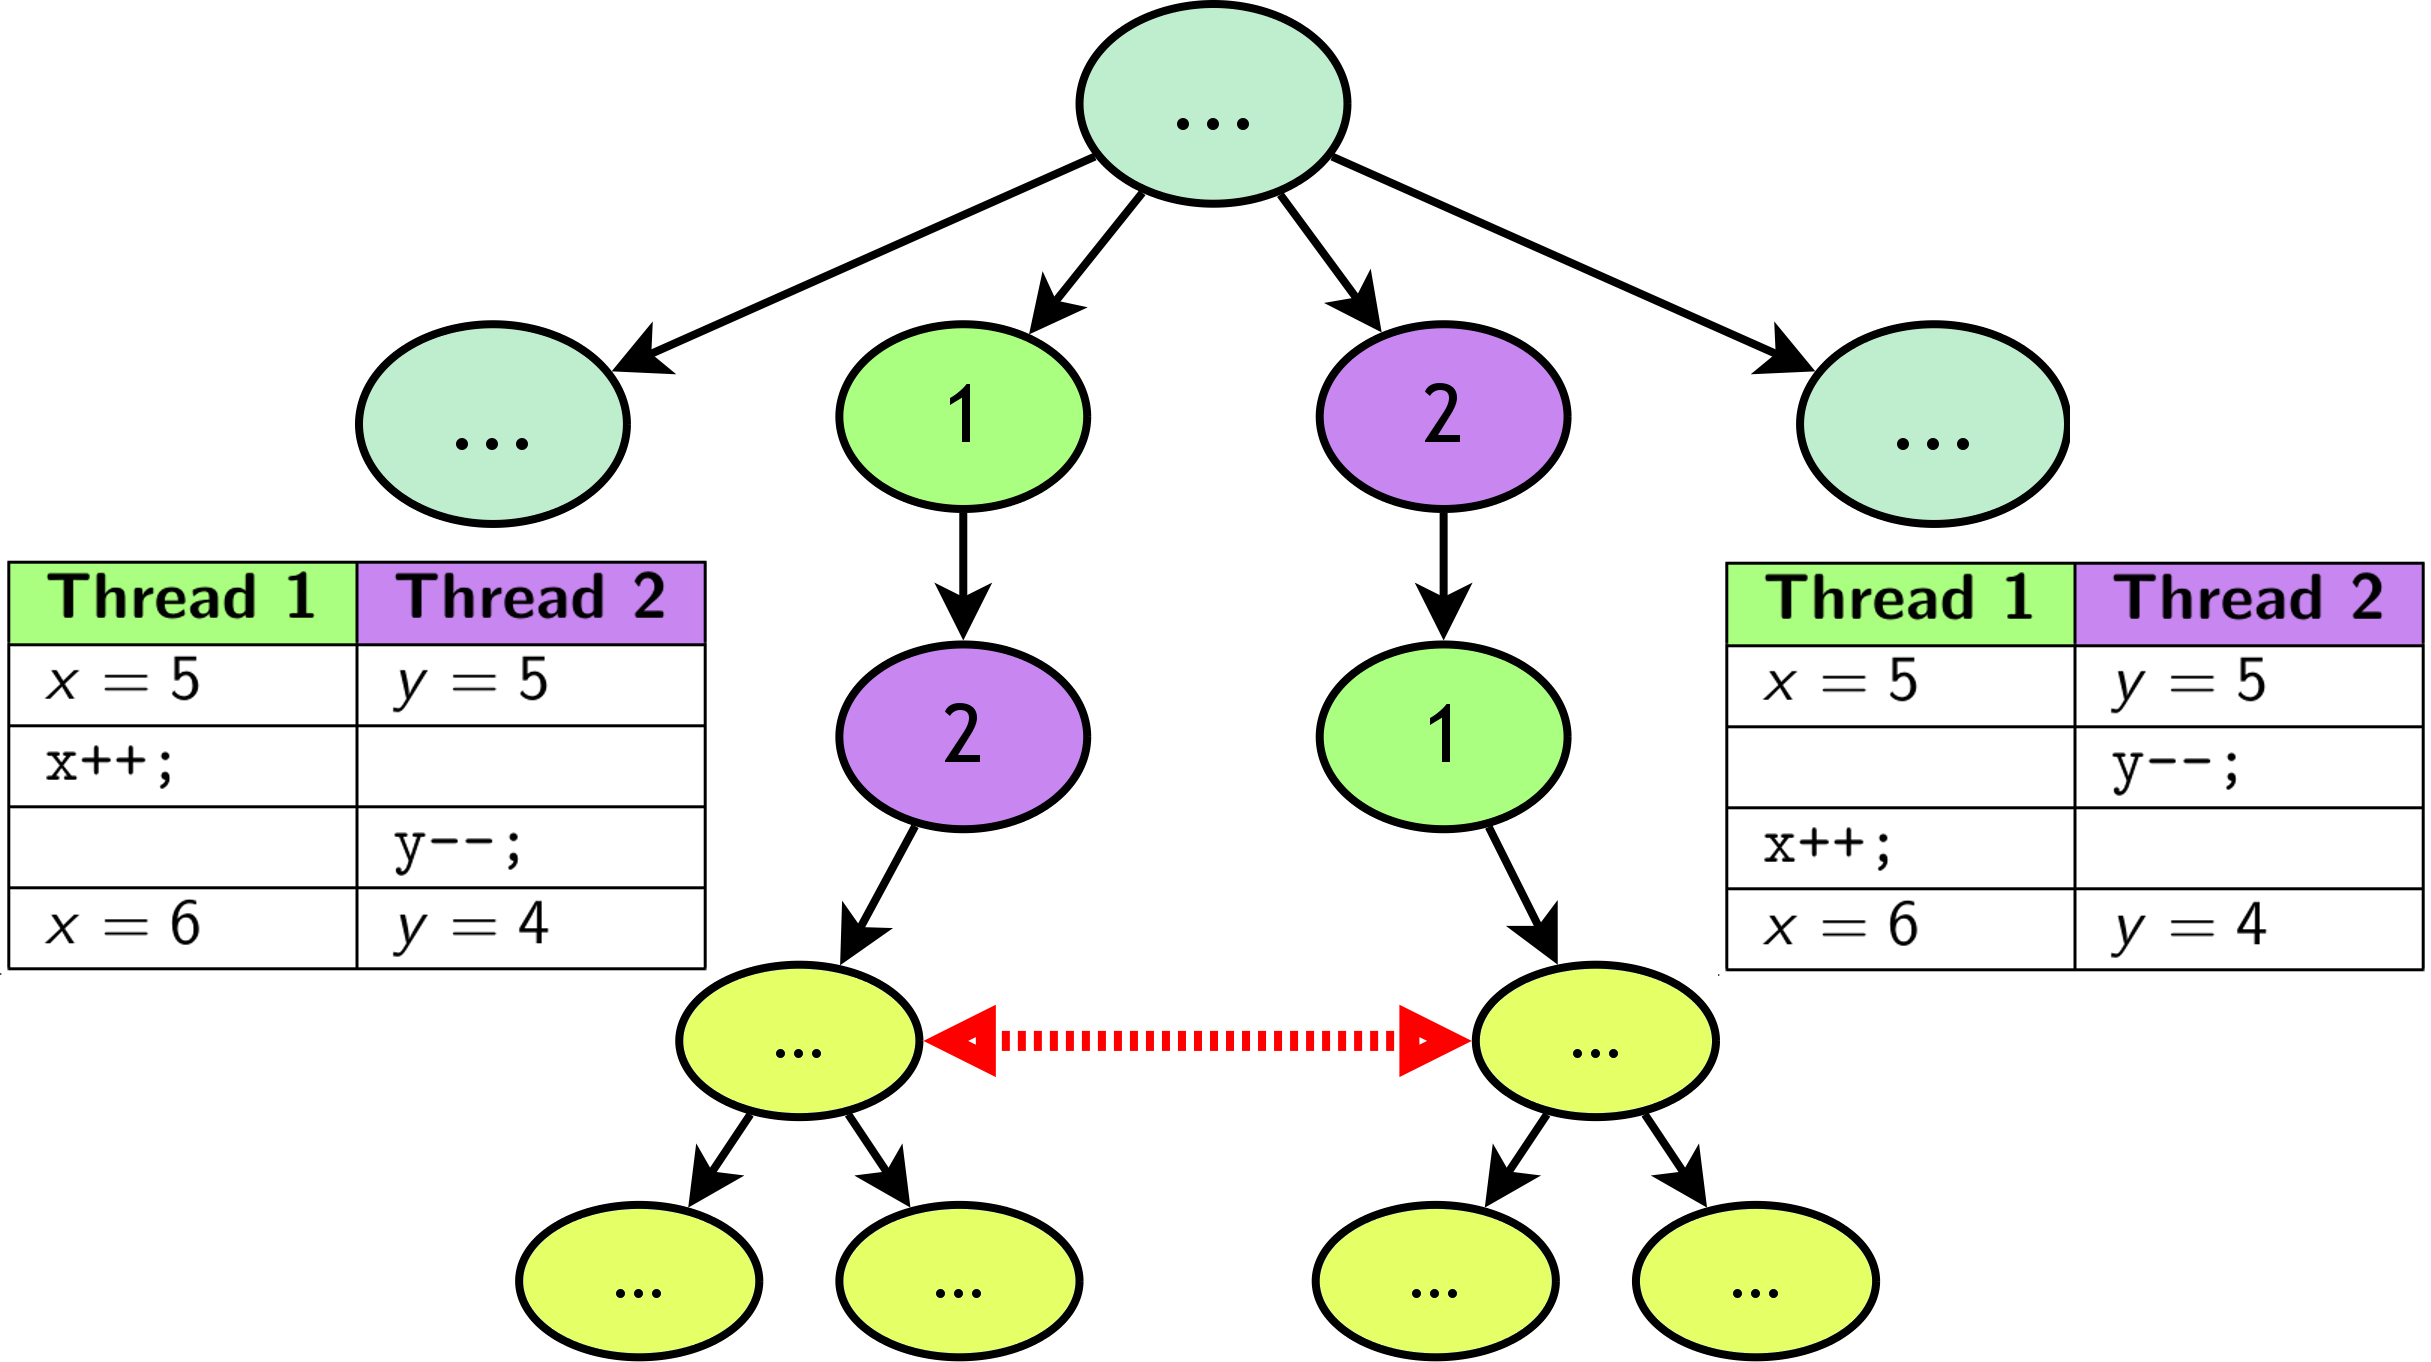
\includegraphics[width=\textwidth]{undiamond1.png}
	\end{center}
\end{frame}
\begin{frame}{State Space Reduction}
	State spaces grow exponentially.
	\begin{itemize}
		\item Fortunately, some sequences result in identical states.
		\item Dynamic Partial Order Reduction\related{Flanagan '05}
		\begin{itemize}
			\item Requires ``memory independence relation'' between transitions.
		\end{itemize}
	\end{itemize}
\end{frame}

\begin{frame}{Shared Memory Conflicts} % slide: ignoring shared memory accesses - venn diagram
	\begin{center}
	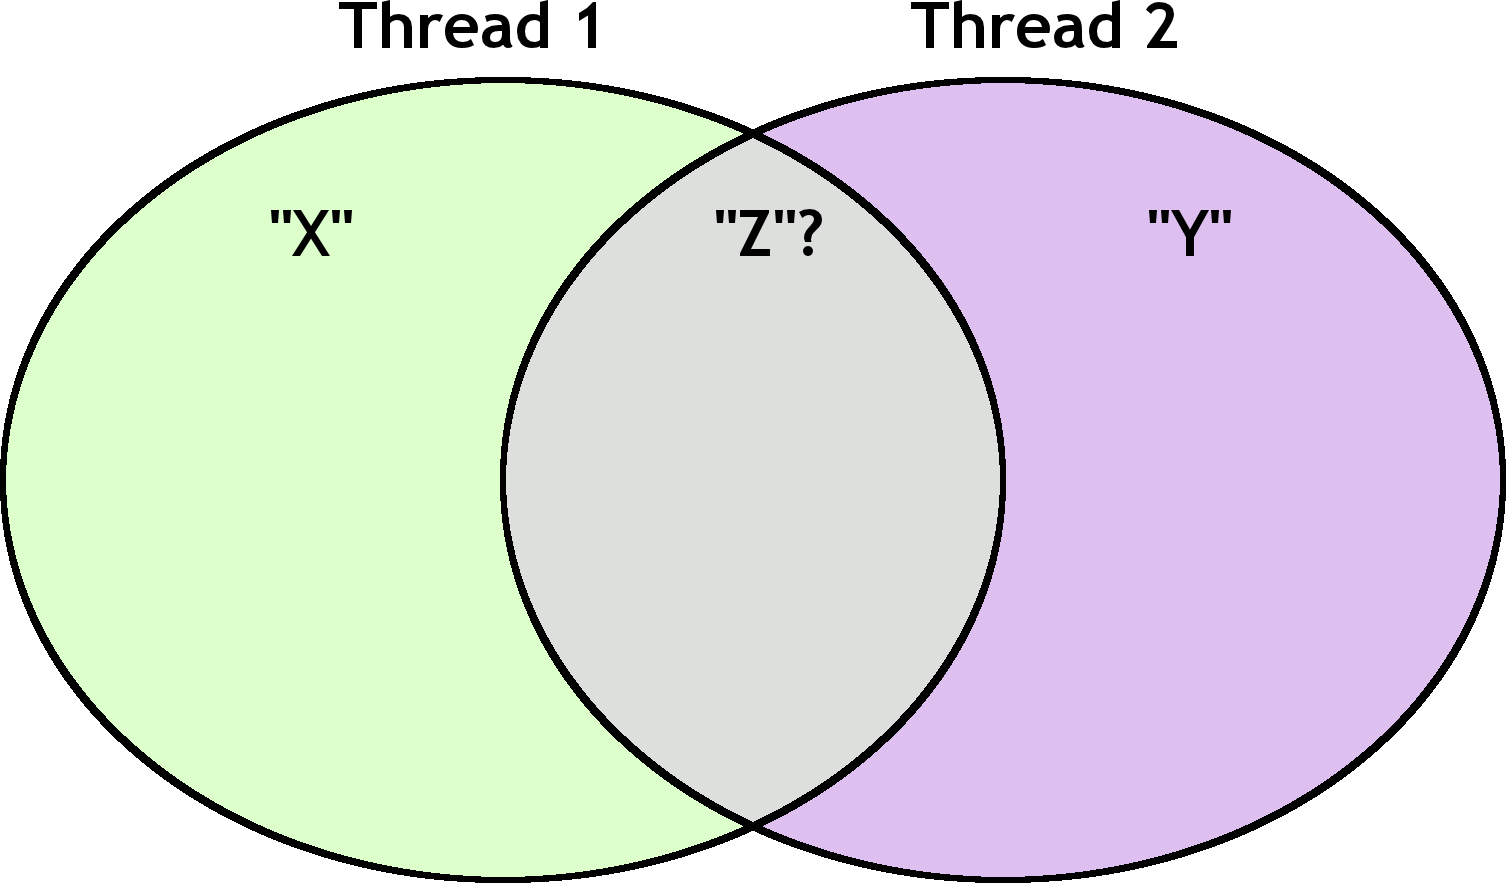
\includegraphics[width=\textwidth]{shm-conflict0.png}
	\end{center}
\end{frame}
\begin{frame}{Shared Memory Conflicts}
	\begin{center}
	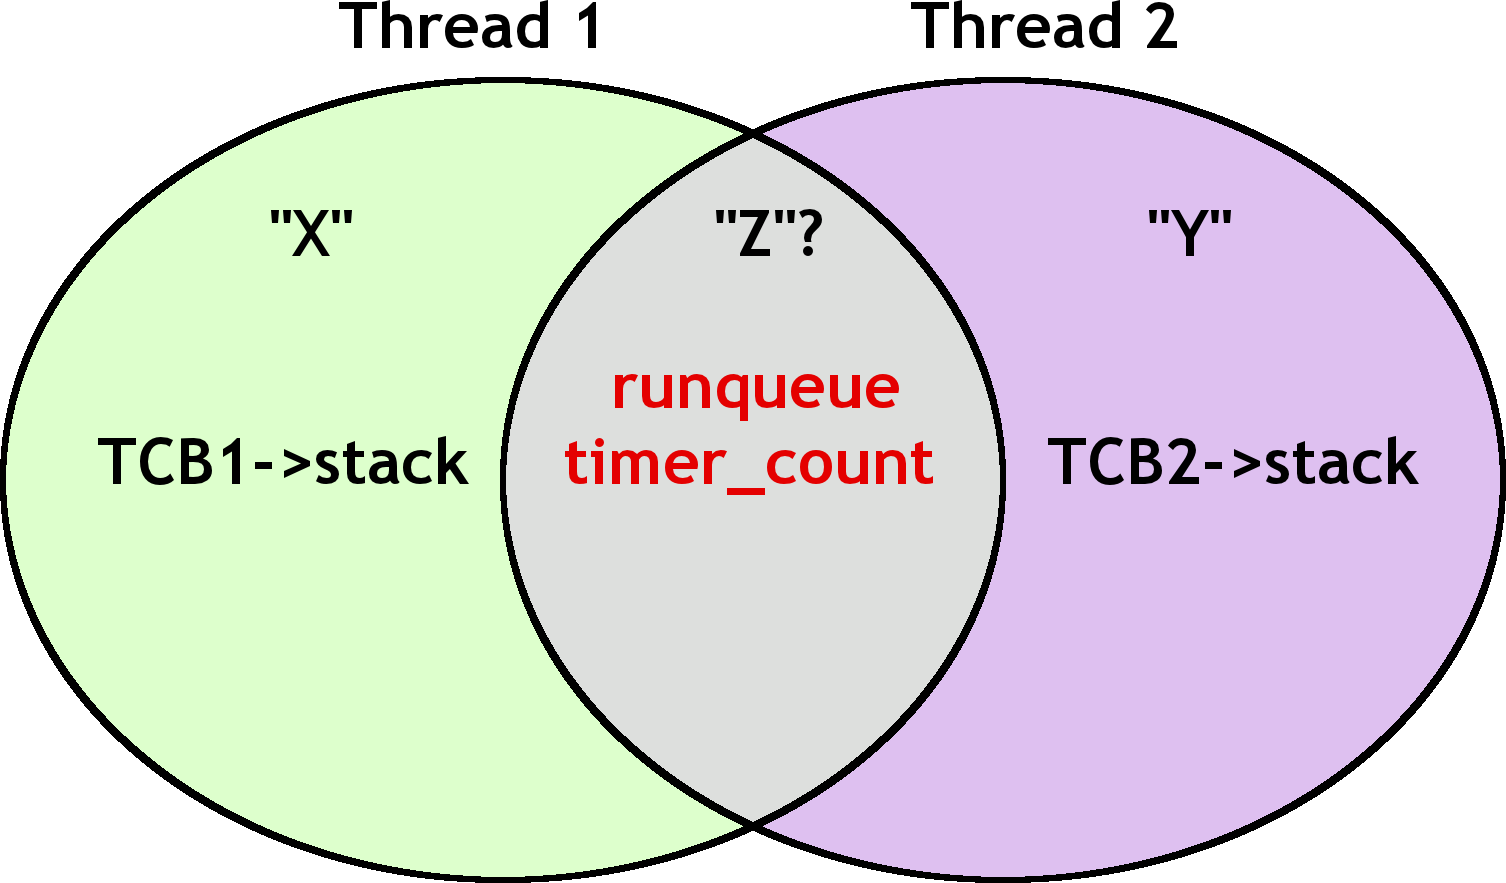
\includegraphics[width=\textwidth]{shm-conflict1.png}
	\end{center}
\end{frame}
\begin{frame}{Shared Memory Conflicts}
	\begin{center}
	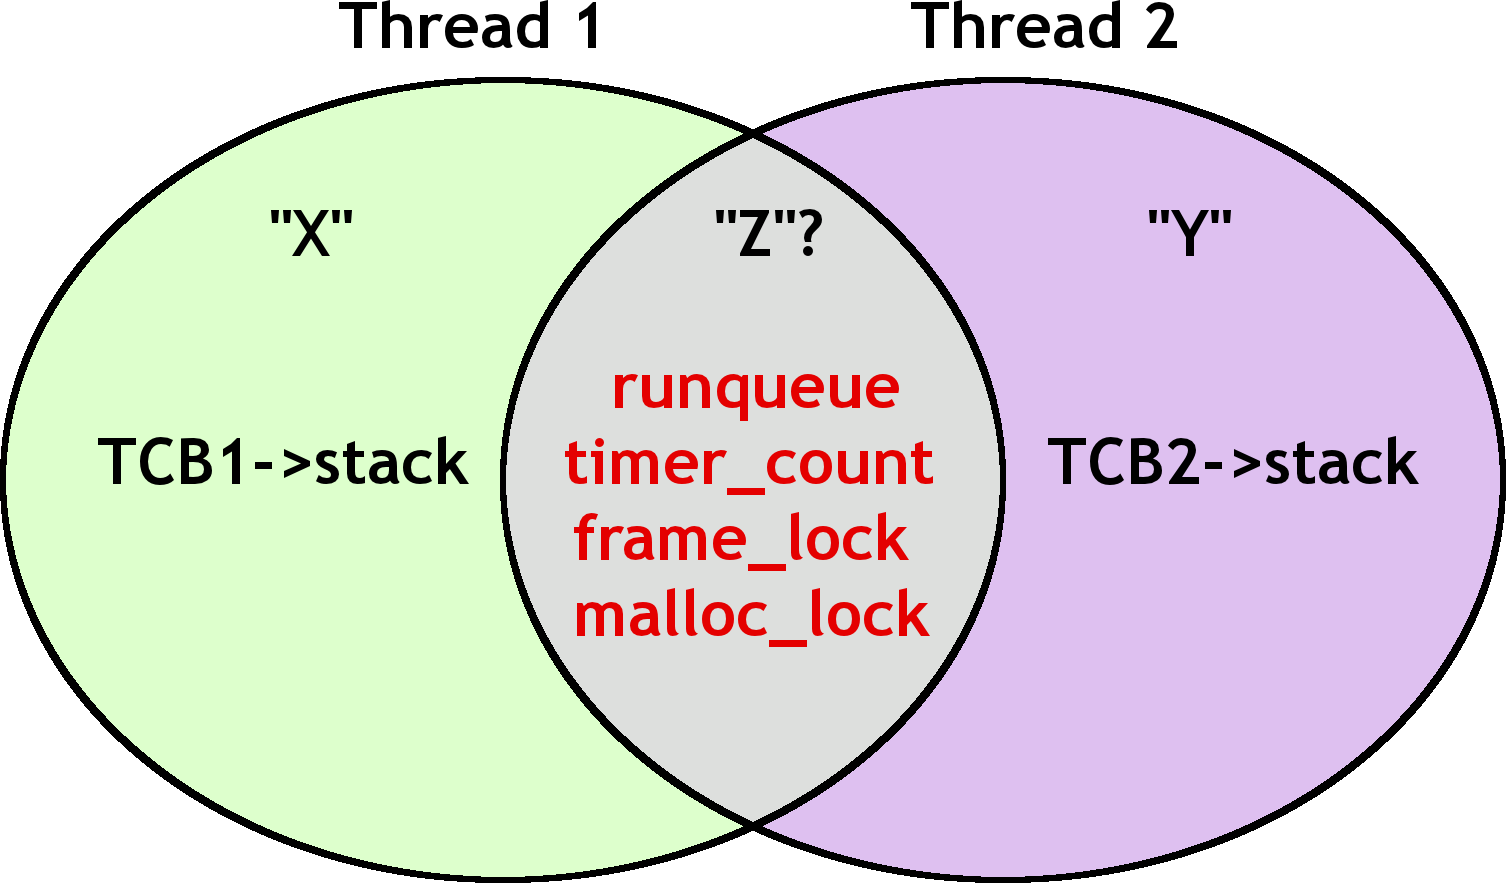
\includegraphics[width=\textwidth]{shm-conflict2.png}
	\end{center}
\end{frame}
\begin{frame}{Shared Memory Conflicts}
	%\textbf{Problem:} Many conflicts we don't care about
	%\begin{itemize}
	%	\item Every transition accesses scheduler state.
	%	\item Many transitions access ``unrelated'' global objects.
	%\end{itemize}
	%\linegap
	\textbf{Solution:} Only consider ``relevant'' memory conflicts.
	\begin{itemize}
		\item Ignore scheduler, global objects assumed to be correct
		\begin{itemize}
			\item Sacrifice ability to test these to efficiently test everything else.
		\end{itemize}
		\item User must specify what to ignore.
	\end{itemize}
\end{frame}

\begin{frame}{Identifying Bugs}
	\textbf{How do we know we've found a bug?}
	\linegap

	% TODO: does this slide want to be multicolumn, with an infinite loop diagram?
	Definite bugs
	\begin{itemize}
		\item Kernel panics / assertion failures
		\item Use-after-free
		\item Deadlock
	\end{itemize}
	Probable bugs
	\begin{itemize}
		\item Infinite loop
		\begin{itemize}
			\item Use structure of execution tree to judge stuckness.
		\end{itemize}
	\end{itemize}
\end{frame}
% slide: other_prob: decide on mutex_lock as opposed to everywhere, but...
% slide: manual shaping - have *user* specify what to focus on (automating intuition)
\begin{frame}{Limiting Decision Points}
\end{frame}
% slide: exciting teaser "i think this is not too far off!"
\begin{frame}{Teaser}
\end{frame}

%%%%%%%%%%%%%%%%%%%%%%%%%%%%%%%%%%%%%%%%%%%%%%%%%%%%%%%%%%%%%%%%%%%%%%%%%%%%%%%%
\section{Evaluation}

%\begin{frame}{Outline}
%	\done{Motivation: Concurrency debugging}
%	\begin{itemize}
%		\item \done{Systematic exploration versus stress testing}
%		\item \done{Challenges of kernel-space}
%	\end{itemize}
%	\linegap
%
%	\done{Tool: Landslide}
%	\begin{itemize}
%		\item \done{Design and interface}
%		\item \done{Addressing challenges}
%	\end{itemize}
%	\linegap
%
%	{\bf Evaluation: Finding Races}
%	\begin{itemize}
%		\item {\bf Student user study}
%		\item {\bf Case study}
%	\end{itemize}
%	\linegap
%
%	Future Work and Conclusion
%\end{frame}

\subsection{User Study}

\begin{frame}{Working with Students} % slide: worked with students - give some time breakdown
	Solicited students in 15-410 to use Landslide on their kernels.
	\begin{itemize}
		\item Can Landslide find bugs ``in the wild''?
		\item How much time does it take to get it working?
	\end{itemize}
	\linegap

	Five groups participated; four got it to work.
	\begin{itemize}
		\item Average instrumentation time 100 minutes (50 to 150)
		%\item Average customisation time 25 minutes (0 to 60)
	\end{itemize}
\end{frame}

\begin{frame}{Landslide Victories} % slide: anecdotes: two deterministic bugs & two races
	All four groups who got it to work found bugs.
	\linegap
	
	Race conditions
	\begin{itemize}
		\item Too many waiters allowed
		\begin{itemize}
			\item One parent thread might block forever
		\end{itemize}
		\item Accidental return to an exited thread
		% Also talk about their vanish/vanish bug
	\end{itemize}
	\linegap

	Deterministic bugs
	\begin{itemize}
		\item Inappropriate idling
		\begin{itemize}
			\item Waiting for a timer tick with no useful work to do
		\end{itemize}
		\item Use-after-free
		\begin{itemize}
			\item Required memory tracking to detect
		\end{itemize}
	\end{itemize}
\end{frame}

\subsection{Case Study}

\begin{frame}{Studying Bugs In-Depth} % slide: "I have built a software smarter than me!" 30-40sec to find
	Worked with two kernels: my own, and one I graded
	\linegap

	``I have made something smarter than me.''
	% Heh, if it were really smarter than me, I wouldn't have had to debug it.
	\begin{itemize}
		\item \texttt{double\_wait} - two parent threads \texttt{wait()} on one exiting child
		\begin{itemize}
			\item Expected: One thread reaps child, the other returns failure
			\item Got: \texttt{failed assertion `nobe->cond\_queue\_next == NULL'}
		\end{itemize}
		\item Previously unknown, not found by stress testing or by TA
	\end{itemize}
\end{frame}

\begin{frame}{Studying Bugs In-Depth} % slide: visual explanation of bug
	% graphic want to be colored TODO
\end{frame}

%%%%%%%%%%%%%%%%%%%%%%%%%%%%%%%%%%%%%%%%%%%%%%%%%%%%%%%%%%%%%%%%%%%%%%%%%%%%%%%%
\section{Conclusion}
%%%%%%%%%%%%%%%%%%%%%%%%%%%%%%%%%%%%%%%%%%%%%%%%%%%%%%%%%%%%%%%%%%%%%%%%%%%%%%%%

%\begin{frame}{Outline}
%	\done{Motivation: Concurrency debugging}
%	\begin{itemize}
%		\item \done{Systematic exploration versus stress testing}
%		\item \done{Challenges of kernel-space}
%	\end{itemize}
%	\linegap
%
%	\done{Tool: Landslide}
%	\begin{itemize}
%		\item \done{Design and interface}
%		\item \done{Addressing challenges}
%	\end{itemize}
%	\linegap
%
%	\done{Evaluation: Finding Races}
%	\begin{itemize}
%		\item \done{Student user study}
%		\item \done{Case study}
%	\end{itemize}
%	\linegap
%
%	{\bf Future Work and Conclusion}
%\end{frame}

%\subsection{Future Work}
\begin{frame}{Promising Directions}
	Top 15-410 students, effectively supervised, can find hard bugs faster.
	\begin{itemize}
		\item Use as a debugging tool may help students learn more.
	\end{itemize}
	\linegap

	After Pebbles\dots
	\begin{itemize}
		\item Potential application to production kernels
		\begin{itemize}
			\item General purpose OSes, device drivers
			% Be ready to field questions about SMP.
		\end{itemize}
	\end{itemize}
	\linegap

	Emphasis on ``steering'' of test parameters by experts
	\begin{itemize}
		\item Perhaps we can automate this steering?
	\end{itemize}
	\linegap
\end{frame}

%\subsection{Summary}
\begin{frame}{Summary}
	\textbf{Systematic exploration in kernel-space}
	\begin{itemize}
		\item Use internal kernel abstractions to understand concurrency behaviour.
		\item Relying on user's knowledge makes testing easier.
	\end{itemize}
	\linegap
	\textbf{Landslide}
	\begin{itemize}
		\item Has potential to be a useful tool for 15-410.
		\item A first step towards sophisticated kernel debugging techniques.
	\end{itemize}

	\linegap
	\linegap
	\begin{center}
	{\scriptsize \em Please hold on. This transit is approaching the Landslide terminal, \\baggage claim, ground transportation, and ticketing.}
	\end{center}
\end{frame}

% slide: bonus slides

\end{document}
%%%%%%%%%%%%%%%%%%%%%%%%%%%%%%%%%%%%%%%%%%%%%%%%%%%%%%%%%%%%%%%%%%%%%%%%%%%%%%%%
%%%%%%%%%%%%%%%%%%%%%%%%%%%%%%%%%%%%%%%%%%%%%%%%%%%%%%%%%%%%%%%%%%%%%%%%%%%%%%%%
%%%%%%%%%%%%%%%%%%%%%%%%%%%%%%%%%%%%%%%%%%%%%%%%%%%%%%%%%%%%%%%%%%%%%%%%%%%%%%%%

\section{Introduction}
\subsection{Introduction}

\subsection{Race Conditions}

% Say: Since I'm no longer a member of course staff, I'm allowed to give away a
% race condition that some of you might have, for the sake of example.

\begin{frame}{Decision Points (``good'' case)}
	\begin{tabular}{|l|l|l}
		\cline{1-2}
		{\bf Thread 1} & {\bf Thread 2} & \\
		\cline{1-2}
		\texttt{spawn\_new\_thread} && \\
		\cline{1-2}
		\texttt{add\_to\_runqueue} && (new thread) \\
		\cline{1-2}
		\texttt{return child->tid} &&  \\
		\cline{1-2}
		& \texttt{vanish} & \\
		\cline{1-2}
		& (TCB gets freed) & (voluntary reschedule) \\
		\cline{1-2}
	\end{tabular}
\end{frame}

\begin{frame}{Decision Points (race condition)}
	\begin{tabular}{|l|l|l}
		\cline{1-2}
		{\bf Thread 1} & {\bf Thread 2} & \\
		\cline{1-2}
		\texttt{spawn\_new\_thread} && \\
		\cline{1-2}
		\texttt{add\_to\_runqueue} && (new thread + preempted) \\
		\cline{1-2}
		& \texttt{vanish} & \\
		\cline{1-2}
		& (TCB gets freed) & (voluntary reschedule) \\
		\cline{1-2}
		\texttt{return child->tid} && (bad!) \\
		\cline{1-2}
	\end{tabular}
\end{frame}

\breakslide{\Large A different way of looking at race conditions\ldots}

\begin{frame}{Execution Tree}
	\begin{center}
		%\includegraphics[width=0.9\textwidth]{threadfork0.png}
	\end{center}
\end{frame}
\begin{frame}{Execution Tree}
	\begin{center}
		%\includegraphics[width=0.9\textwidth]{threadfork05.png}
	\end{center}
\end{frame}
\begin{frame}{Execution Tree}
	\begin{center}
		%\includegraphics[width=0.9\textwidth]{threadfork1.png}
	\end{center}
\end{frame}
\begin{frame}{Execution Tree}
	\begin{center}
		%\includegraphics[width=0.9\textwidth]{threadfork2.png}
	\end{center}
\end{frame}

\begin{frame}{Decision Points} % : duplicate slide with later
	A {\bf decision point} is\ldots

	\linegap
	A code location where being preempted causes different behaviour.
	\begin{itemize}
		\item Intuitively: Somewhere that interesting interleavings can happen around.
	\end{itemize}
	Examples:
	\begin{itemize}
		\item A new thread becomes runnable
		\item Voluntary reschedule (e.g. \texttt{yield}, \texttt{cond\_wait})
		\item Synchronization primitives
	\end{itemize}
	% Say: We'll revisit this later.
\end{frame}

% Say: Obviously we want to be able to always run the third path. But knowing
% that ahead of time is impossible.
% Say: Okay, now what if we could build a tool that could ``systematically''
% explore this tree, and find the branch with the bug in it? What would such a
% tool need to be able to do?

%%%%%%%%%%%%%%%%%%%%%%%%%%%%%%%%%%%%%%%%%%%%%%%%%%%%%%%%%%%%%%%%%%%%%%%%%%%%%%%%
%%%%%%%%%%%%%%%%%%%%%%%%%%%%%%%%%%%%%%%%%%%%%%%%%%%%%%%%%%%%%%%%%%%%%%%%%%%%%%%%
%%%%%%%%%%%%%%%%%%%%%%%%%%%%%%%%%%%%%%%%%%%%%%%%%%%%%%%%%%%%%%%%%%%%%%%%%%%%%%%%

\section{Systematic Testing}

\breakslide{\Large Systematic Testing}

\begin{frame}{Systematic Testing}
	\textbf{Systematic testing} is:
	\begin{itemize}
		\item Systematically enumerating different interleavings
		\begin{itemize}
			\item Intuitively: Generate many ``tabular execution traces''
		\end{itemize}
		\item Exploring all branches in these trees
		\begin{itemize}
			\item (by controlling scheduling decisions at decision points)
		\end{itemize}
		\item In practice: Depth-first search of branches
	\end{itemize}
\end{frame}

\subsection{Requirements}


\begin{frame}{Execution Tree Exploration}
	Important point: When does a branch end?
	\begin{itemize}
		\item All threads run to completion, or
		\item A bug is detected % Say: more on this later.
	\end{itemize}
	{\bf Backtracking}:
	\begin{itemize}
		\item Identify a decision point to choose differently
		\item Reset machine state and start over
		\item Replay test from the beginning, with different choices
	\end{itemize}
\end{frame}


\begin{frame}{More on Decision Points}
	Important point: What does ``all possible interleavings'' mean?

	\linegap
	One extreme: Decide at every instruction
	\begin{itemize}
		\item Good news: Will find every possible race condition.
		\item Bad news: Runtime of test will be impossibly large.
	\end{itemize}
	\linegap

	Other extreme: Nothing is a decision point
	\begin{itemize}
		\item Good news: Test will finish quickly.
		\item Bad news: Only one execution was checked for bugginess.
		\item Bad news: No alternative interleavings explored.
		\begin{itemize}
			\item Makes ``no race found'' a weak claim.
		\end{itemize}
	\end{itemize}
\end{frame}

\begin{frame}{More on Decision Points}
	Sweet spot: Insert a thread switch everywhere it ``might matter''.

	\linegap
	When do we fear being preempted?
	\begin{itemize}
		\item New threads becoming runnable (\texttt{fork}, \texttt{cond\_signal}, etc)
			\begin{itemize}
				\item Preemptions may cause it to run before we're ready
			\end{itemize}
		\item Synchronization primitives (\texttt{mutex\_lock}, etc)
			\begin{itemize}
				\item If used improperly\ldots
			\end{itemize}
		\item Unprotected shared memory accesses % Say: more on this later.
			\begin{itemize}
				\item May result in data structure corruption
			\end{itemize}
	\end{itemize}
	\linegap

	Finding the sweet spot is a joint effort between programmer and tool. (More on this later.)
\end{frame}

\subsection{Challenges}

\begin{frame}{Controlling Scheduling Decisions}
	Control over sources of nondeterminism
	\begin{itemize}
		\item Device interrupts/input
			\begin{itemize}
				\item Disk drivers: when disk reads finish
				\item Ethernet drivers: when packets arrive
			\end{itemize}
		\item To control thread switches in a 410 kernel, vary when clock ticks happen.
	\end{itemize}
\end{frame}

\begin{frame}{Memory Interposition}
	In order to find use-after-free, need to know:
	\begin{itemize}
		\item When objects are \texttt{free()}d
		\item When threads access shared memory in the heap
	\end{itemize}
	\linegap

	Solution: Keep track of all memory events
	\begin{itemize}
		\item All calls to \texttt{malloc}/\texttt{free}
		\item All shared memory reads/writes
	\end{itemize}
\end{frame}

%%%%%%%%%%%%%%%%%%%%%%%%%%%%%%%%%%%%%%%%%%%%%%%%%%%%%%%%%%%%%%%%%%%%%%%%%%%%%%%%

\subsection{State Space Explosion}

\begin{frame}{State Space Explosion}
	State spaces grow exponentially
	\begin{itemize}
		\item With $d$ decision points, $k$ runnable threads, size $d^k$.
		\item Threatens our ability to explore everything.
		\item Fortunately, some sequences result in identical states.
	\end{itemize}
	\linegap

	{\bf Partial Order Reduction} can help.
	\begin{itemize}
		\item Complicated algorithm; ask me later for details.
		\item Intuitive explanation follows.
	\end{itemize}
\end{frame}

\begin{frame}{State Space Explosion}
	\begin{center}
	%\includegraphics[width=\textwidth]{undiamond0.png}
	\end{center}
\end{frame}
\begin{frame}{State Space Explosion}
	\begin{center}
	%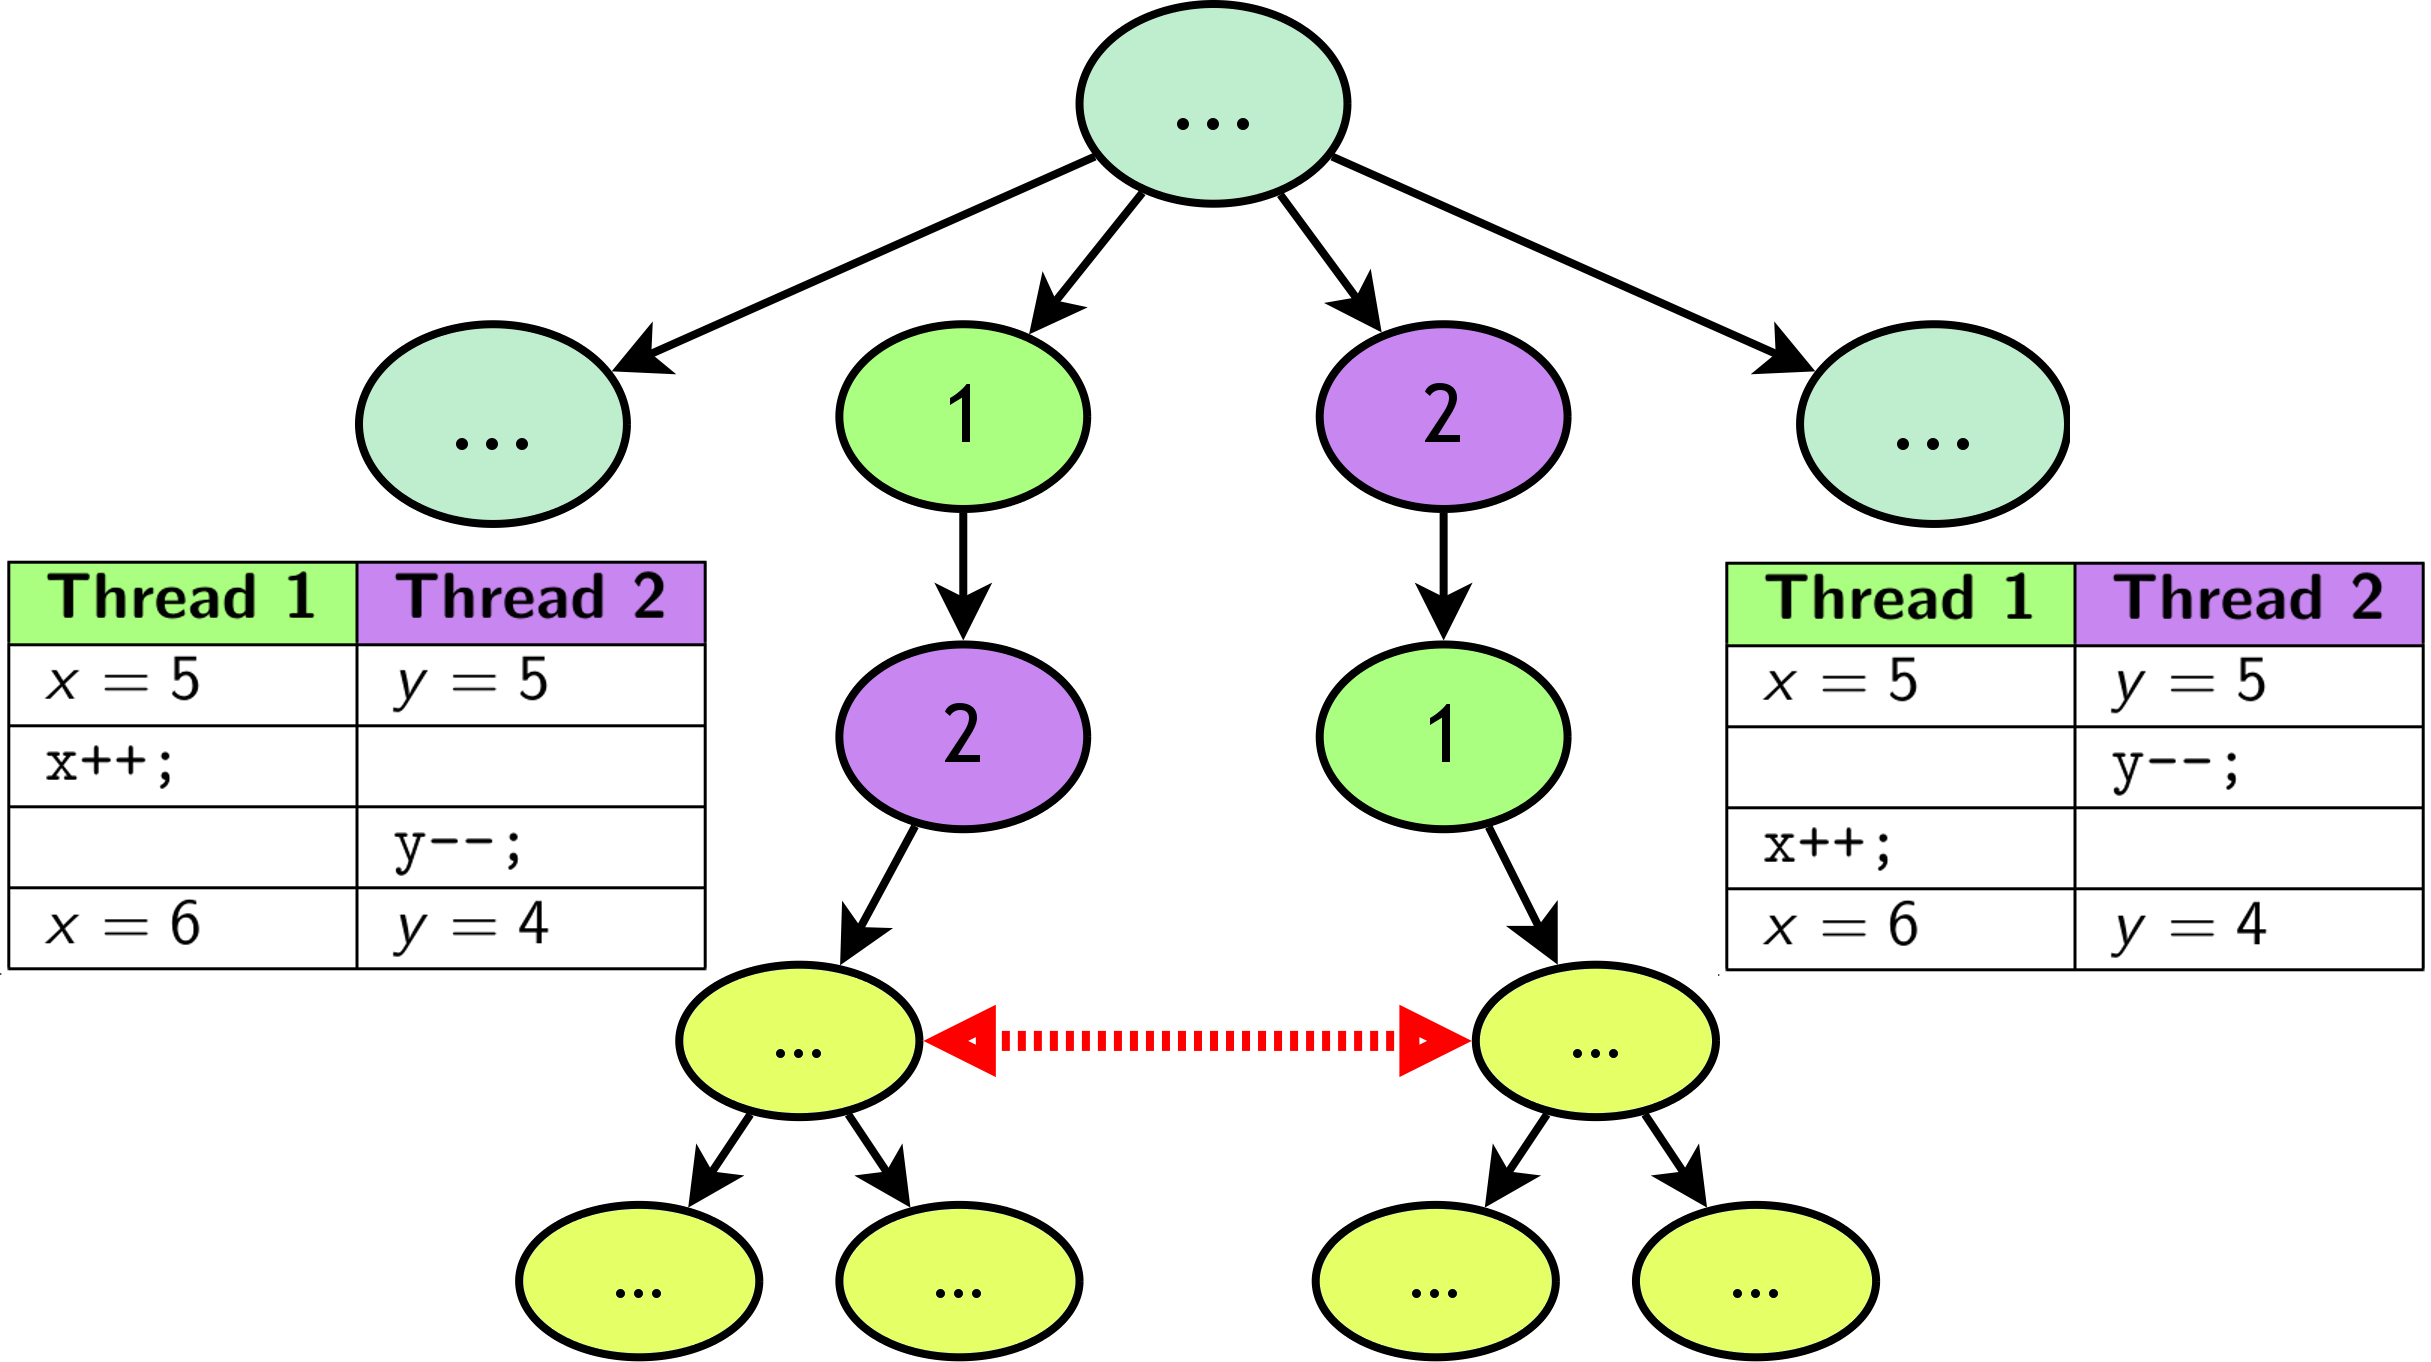
\includegraphics[width=\textwidth]{undiamond1.png}
	\end{center}
\end{frame}
\begin{frame}{State Space Explosion}
	\begin{center}
	%\includegraphics[width=\textwidth]{diamond1.png}
	\end{center}
\end{frame}

%%%%%%%%%%%%%%%%%%%%%%%%%%%%%%%%%%%%%%%%%%%%%%%%%%%%%%%%%%%%%%%%%%%%%%%%%%%%%%%%
%%%%%%%%%%%%%%%%%%%%%%%%%%%%%%%%%%%%%%%%%%%%%%%%%%%%%%%%%%%%%%%%%%%%%%%%%%%%%%%%
%%%%%%%%%%%%%%%%%%%%%%%%%%%%%%%%%%%%%%%%%%%%%%%%%%%%%%%%%%%%%%%%%%%%%%%%%%%%%%%%

\section{Landslide}

\breakslide{\Huge Landslide}

\begin{frame}{About The Project}
	5th year MS since June 2011 % Say: planning to finish this may, hopefully

	\linegap
	Working with Garth Gibson, Jiri Simsa

	\linegap
	{\bf Landslide}: Shows that your Pebbles are not as stable as you thought.
\end{frame}

%%%%%%%%%%%%%%%%%%%%%%%%%%%%%%%%%%%%%%%%%%%%%%%%%%%%%%%%%%%%%%%%%%%%%%%%%%%%%%%%

\subsection{How Landslide Works}

\begin{frame}{Landslide in Simics}
	As a Simics module, Landslide knows:
	\begin{itemize}
		\item Every instruction the kernel executes
		\item Every memory address the kernel reads/writes
	\end{itemize}
	\linegap
	Artificially causes timer interrupts

	\linegap
	Checkpointing/backtracking via Simics bookmarks
\end{frame}

\begin{frame}{Anatomy}
	\begin{center}
	%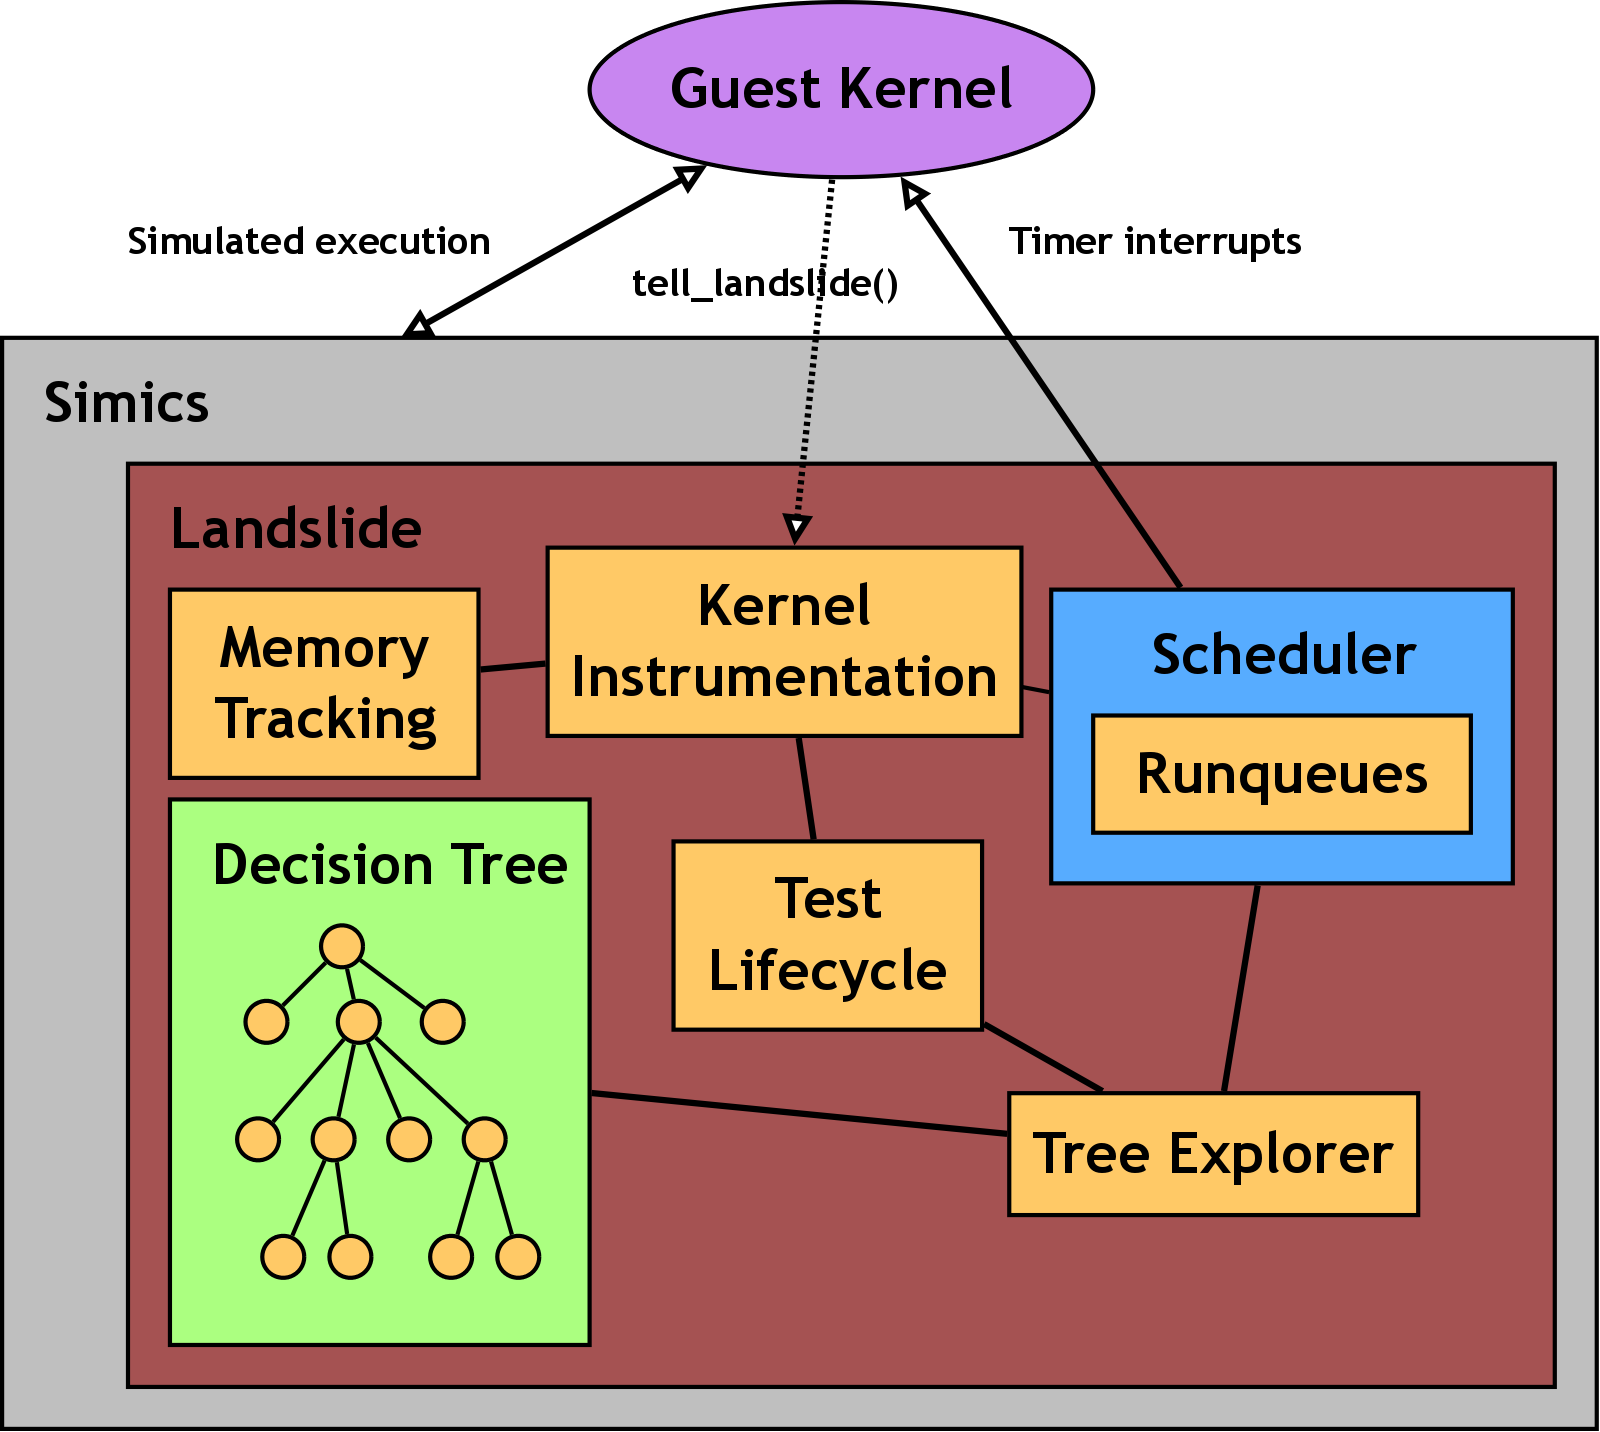
\includegraphics[width=0.6\textwidth]{landslide.png}
	\end{center}
\end{frame}

\begin{frame}{Identifying Bugs}
	Landslide can {\em definitely discover}:
	\begin{itemize}
		\item Kernel panics % Say: note: the better your asserts are..!
		\item Deadlock
		\item Use-after-free / double-free
	\end{itemize}
	Landslide can {\em reasonably suspect}:
	\begin{itemize}
		\item Memory leak
		\item Progress sense (halting problem)
	\end{itemize}
\end{frame}

%%%%%%%%%%%%%%%%%%%%%%%%%%%%%%%%%%%%%%%%%%%%%%%%%%%%%%%%%%%%%%%%%%%%%%%%%%%%%%%%

\subsection{Using Landslide}

\breakslide{\Large Using Landslide}

\begin{frame}{In Which Ben Offers Help}
	% Say: So, this wasn't just a research talk
	This is something you can try!
	\linegap

	Mutual benefit
	\begin{itemize}
		\item Landslide may help you find bugs
		\item You may help Ben evaluate his thesis project
	\end{itemize}
\end{frame}

\begin{frame}{Keeping It Real}
	Finding race conditions is hard for humans.

	\linegap
	It is hard for computer programs too.

	\linegap
	Landslide is not an oracle.
\end{frame}

\begin{frame}{Annotating Your Kernel}
	Step 1
	\begin{center}
		%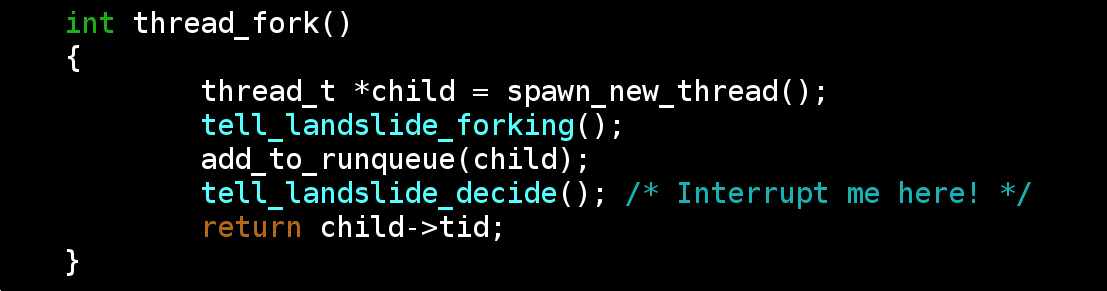
\includegraphics[width=0.9\textwidth]{tell_landslide.png}
	\end{center}
	Your kernel needs to say when certain events happen:
	\begin{itemize}
		\item When do threads become runnable / descheduled?
		\item When does the scheduler switch threads?
	\end{itemize}
	\linegap

	\framebox{Time estimate: 40 minutes}
\end{frame}

\begin{frame}{Configuring Landslide}
	Step 2
	\begin{center}
		%\includegraphics[width=0.8\textwidth]{config-landslide.png}
	\end{center}
	Edit \texttt{config.landslide} with some details and tweaks

	Fill in two implementation-dependent C functions in Landslide ($\le$10 lines)
	% Say: Which depend on your kernel's specific implementation
	\linegap

	\framebox{Time estimate: 60 minutes}
\end{frame}

\begin{frame}{Configuring Decision Points}
	Landslide automatically identifies a minimal set of decision points.
	\begin{itemize}
		\item It might find bugs.
		\item It might overlook more fine-grained interleavings.
	\end{itemize}
	With help from you, it could find more.
	\begin{itemize}
		\item Optional annotation: \texttt{tell\_landslide\_decide()}
		\item Hints to where a context switch should be forced.
		\item Inside every call to \texttt{mutex\_lock}\ldots
	\end{itemize}
\end{frame}

\breakslide{\Large Quick Demo}


%\begin{frame}{Decision Points (noticing a theme here?)}
%	Landslide is {\bf false negative}-oriented.
%	\begin{itemize}
%		\item If Landslide reports a bug, there is a bug for sure.
%			% Say: Well, except progress sense might be wrong.
%		\item If not,
%			\begin{itemize}
%				\item Maybe there was no race, or
%				\item Maybe your decision points were not granular enough.
%			\end{itemize}
%	\end{itemize}
%\end{frame}
%\begin{frame}{Decision Points (noticing a theme here?)}
%	Sometimes the default set will work.
%
%	Sometimes you need to tweak\ldots
%	\begin{itemize}
%		\item Ignore certain global mutexes
%		\item Whitelist or blacklist entire syscalls
%		\item (get creative)
%	\end{itemize}
%	Intuitively: focusing Landslide on relevant parts of the kernel.
%\end{frame}

%%%%%%%%%%%%%%%%%%%%%%%%%%%%%%%%%%%%%%%%%%%%%%%%%%%%%%%%%%%%%%%%%%%%%%%%%%%%%%%%

\subsection{User Study}

\begin{frame}{In Which Ben Offers Help - Warning}
	\textbf{If you are already struggling, this will not ``save'' you.}
	\begin{itemize}
		\item False-negatives: not guaranteed to find races at all
		\item Research-quality: possibly difficult to integrate with your kernel
		\item Finishing the kernel project is more important.
	\end{itemize}
	You should:
	\begin{itemize}
		\item Be expecting an A or B
		\item Be able to turn in without late days (if you really had to)
		\item Be looking for\ldots
			\begin{itemize}
				\item That ``one pesky race''
				\item A race that stress-testing missed
				\item Or just familiarity with a new technique
			\end{itemize}
	\end{itemize}
\end{frame}

\begin{frame}{In Which Ben Offers Help}
	Your kernel
	\begin{itemize}
		\item Must load the shell and run programs
		\item \texttt{fork},
			\texttt{exec},
			\texttt{vanish},
			\texttt{wait},
			\texttt{readline}
		\item Must never spin-wait (see hurdle form!)
		\item Should \texttt{assert()} important invariants
		\begin{itemize}
			\item Think of \texttt{panic()} as \texttt{tell\_landslide\_bug()}
		\end{itemize}
	\end{itemize}
\end{frame}

\begin{frame}{In Which Ben Offers Help}
	User study next week, starting Monday

	\linegap
	Expect to spend:
	\begin{itemize}
		\item Up to 4 hours, just to try it out.
		\item 6-8 hours, if you find a bug and track it down.
		\item More, for multiple bugs or the truly dedicated\ldots
	\end{itemize}
	\linegap

	Give feedback (intuitive? frustrating? found bugs?)

	\linegap
	{\bf Watch \texttt{410.announce} for details!}
\end{frame}

\subsection{End}
\breakslide{\Large Questions?}

%%%%%%%%%%%%%%%%%%%%%%%%%%%%%%%%%%%%%%%%%%%%%%%%%%%%%%%%%%%%%%%%%%%%%%%%%%%%%%%%
%%%%%%%%%%%%%%%%%%%%%%%%%%%%%%%%%%%%%%%%%%%%%%%%%%%%%%%%%%%%%%%%%%%%%%%%%%%%%%%%
%%%%%%%%%%%%%%%%%%%%%%%%%%%%%%%%%%%%%%%%%%%%%%%%%%%%%%%%%%%%%%%%%%%%%%%%%%%%%%%%


% \section{Conclusion}
% \subsection{Conclusion}
% 
% \begin{frame}{Summary}
% 	\begin{itemize}
% 		\item
% 	\end{itemize}
% \end{frame}

%\begin{frame}{Partial Order Reduction}
%	\begin{center}
%	The next 6 slides won't be on the exam.
%
%		\Huge \dbend
%	\end{center}
%\end{frame}
%
%\begin{frame}{Partial Order Reduction}
%	A {\bf transition} is\ldots
%	\begin{itemize}
%		\item The sequence of instructions executed between choice points.
%	\end{itemize}
%	To express concurrency between transitions:
%	% Say: As a prerequisite for this algorithm, we need to build two sets to express the concurrency relations between the transitions
%	\begin{itemize}
%		\item Independence relation
%		\item Happens-before relation
%	\end{itemize}
%	% Say: This is hard, and I don't expect you to understand it during this lecture; you won't be tested on it or anything. My goal in presenting it is to convey how intensely cool the algorithm is, and hopefully you will keep thinking about it later. I'd be happy to answer questions about it later.
%\end{frame}
%
%\begin{frame}[fragile]{Partial Order Reduction - Independence Relation}
%	\begin{columns}[l]
%		\column{0.5\textwidth}
%		\begin{center}
%		\begin{verbatim}
%		void thread_A() {
%		    foo = 42;
%		}
%		void thread_B() {
%		    if (bar == 1337)
%		        print "Hello"
%		}
%		\end{verbatim}
%		\end{center}
%		\linegap
%
%		$A$ and $B$ are {\bf independent}.
%		\column{0.5\textwidth}
%		\begin{center}
%		\begin{verbatim}
%		void thread_A() {
%		    foo = 42;
%		}
%		void thread_C() {
%		    if (foo == 1337)
%		        print "Hello"
%		}
%		\end{verbatim}
%		\end{center}
%		\linegap
%
%		$A$ and $C$ {\bf conflict}.
%	\end{columns}
%\end{frame}
%
%\begin{frame}{Partial Order Reduction - Independence Relation}
%	Consider a trace of all shared memory reads/writes
%
%	\linegap
%	Two transitions (instruction sequences) $A$ and $B$ are independent iff:
%	\begin{itemize}
%		\item $Writes(A) \cap Writes(B) = \emptyset$
%		\item $Writes(A) \cap Reads(B) = \emptyset$
%		\item $Reads(A) \cap Writes(B) = \emptyset$
%	\end{itemize}
%\end{frame}
%
%\begin{frame}{Partial Order Reduction - Happens-before Relation}
%	\begin{columns}[l]
%		\column{0.5\textwidth}
%		%\includegraphics[width=\textwidth]{hb.png}
%		\column{0.5\textwidth}
%		Is a transition ``enabled'' by a previous one?
%		\begin{itemize}
%			\item $A$ enables $B$
%			\item $B$ enables $C$ (same thread)
%			\item $B$ enables $D$
%		\end{itemize}
%%		Transitive closure
%%		\begin{itemize}
%%			\item $HB^* = \{AB, AC, AD, BC, BD\}$
%%		\end{itemize}
%		$C$ and $D$ are {\bf concurrent}!
%	\end{columns}
%\end{frame}
%
%\begin{frame}{Partial Order Reduction - Tagging}
%	Run POR at the end of each branch
%	\begin{itemize}
%		\item Identify which branches to explore next
%		\item Tag only a subset of all branches (hopefully)
%	\end{itemize}
%\end{frame}
%
%\begin{frame}{Partial Order Reduction - Tagging}
%	For each transition $T$, find an {\bf evil ancestor} $E$:
%	\begin{itemize}
%		\item $E$ and $T$ are concurrent.
%		\item $E$ and $T$ are not independent.
%		\item Intuitively: $T$ and $E$ could be reordered, and might behave differently.
%	\end{itemize}
%	Find a {\bf good sibling} $G$ of $E$:
%	\begin{itemize}
%		\item $G$ is the same thread as $T$
%		% Say: (if no such sibling, all siblings)
%		\item Intuitively: Find a branch in which $T$ runs before $E$.
%	\end{itemize}
%	Explore tagged branches depth-first.
%\end{frame}
%
%\begin{frame}{Partial Order Reduction}
%	\begin{center}
%		{\Huge \dbend}
%		\linegap
%		\linegap
%		\linegap
%
%		Feel free to ask me about this later.
%	\end{center}
%\end{frame}


%%%%%%%%%%%%%%%%%%%%%%%%%%%%%%%%%%%%%%%%%%%%%%%%%%%%%%%%%%%%%%%%%%%%%%%%%%%%%%%%

%\subsection{Other Dynamic Techniques}
%
%\begin{frame}{Heuristic-Based Searching}
%	% Say: Note that this is beyond the scope of my personal project.
%	Maybe the tree is too big to search anyway?
%
%	\linegap
%	Search {\em most likely} branches first.
%	\begin{itemize}
%		\item ``Iterative Context Bounding''
%		\footnote{Microsoft Research - CHESS - Musuvathi et al.}
%		\begin{itemize}
%			\item Insight: Races tend to show up with few forced context switches.
%			\item Search branches with fewer preemptions first.
%		\end{itemize}
%		\item Find behaviours that are typical of buggy software.
%		\footnote{Stanford University - Dawson Engler}
%		\begin{itemize}
%			\item Different behaviour in different branches.
%				% Say: different all the time: no. different rarely: yes.
%			\item Use suspicious memory accesses as future choice points.
%		\end{itemize}
%	\end{itemize}
%	\linegap
%	Open research field, possibly my future work.
%\end{frame}
%
%% Say: I'm going to take a break from talking about systematic exploration to talk about other types of dynamic race detection - FIXME: if these slides fit in 60min.
%\begin{frame}{Data Race Detection}
%	Requires happens-before set and ``lock set''
%	\linegap
%
%	Two memory accesses $m_1$ and $m_2$ are a data race iff:
%	\begin{itemize}
%		\item Read/write or write/write to the same address, and
%		\item $(m_1,m_2) \not\in HB$, and
%		\item $Lock(m_1) \cap Lock(m_2) = \emptyset$
%	\end{itemize}
%\end{frame}
%\begin{frame}{Data Race Detection}
%	Data race detection vs systematic exploration
%	\begin{itemize}
%		\item More false positives
%			\begin{itemize}
%				\item (but still good style-checking!)
%			\end{itemize}
%		\item No false negatives
%		\item Still unable to find some types of bugs
%	\end{itemize}
%	\linegap
%	Hybrid approach? (future research)
%\end{frame}

% vim: foldmethod=indent
